% v1.7 - 2014-11-18
% - bib fixes: now using biber instead of bibtex (thanks felix)
% - compile now with pdflatex -> biber -> pdflatex
% v1.6 - 2013-05-13
% - bibliography headers fixed - thanx lorenz lehmann
% - high quality titlepage - thanx thomas graf
% - removed separation of online and offline references -> style 1.4a
% v1.5 - 2013-01-16

\documentclass[twoside,11pt,titlepage,a4paper,english,bibliography=totocnumbered,listof=numbered]{scrbook}

% Template Style
% =========================================================================
% = SNET THESIS TEMPLATE STYLE
% =========================================================================

% http://www.snet.tu-berlin.de
% ------------------------
% Adapted version from http://hci.rwth-aachen.de/karrer_thesistemplate (Thorsten Karrer)
% Further adaptions for http://www.elearn.rwth-aachen.de (Sascha Hoellger)
% Further adaptions for SNET @ TU Berlin by Sebastian Göndör (sebastian.goendoer@tu-berlin.de)


% =========================================================================
% = CHANGELOG
% =========================================================================

% [0.1.4b]
% backend=biber added in line 139
% 
% [0.1.4a]
% title page: image logo sizes and margins adjusted to printable area
% removed separation of online and offline references
%
% [0.1.3]
% wider text body
% added "school" to the titlepage
% paragraph indents
% correctly placed footnote graphics
% 
% [0.1.2]
% new titlepage
% some minor fixes
% 
% [0.1.1]
% changed titlepage logo
% added listoffigures and listoftables
% excluded abstract from toc
% no (roman) numbering for frontmatter
% 
% [0.1]
% adapted version 0.991b from sascha hoellger @ rwth aachen


% =========================================================================
% = MISC
% =========================================================================

\usepackage{a4wide}					% 
\usepackage{verbatim}				% 
\usepackage[toc,page]{appendix}			% 
\usepackage[withpage]{acronym}			% 
\usepackage{amsthm}				% Definitions


% =========================================================================
% = COLORS
% =========================================================================

\usepackage{xcolor}					% Colors
\definecolor{LightBlue}{rgb}{0.55,0.55,1}
\definecolor{DarkBlue}{rgb}{0.2,0.2,0.5}
\definecolor{Maroon}{rgb}{0.6,0.15,0.2}
\definecolor{DarkRed}{rgb}{0.71,0.12,0.07}
\definecolor{DarkGreen}{rgb}{0.2,0.6,0.2}
\definecolor{LightGray}{rgb}{0.8,0.8,0.8}

% =========================================================================
% = PAGE LAYOUT
% =========================================================================

\usepackage{geometry}
\geometry{inner=3cm, outer=2cm, bottom=4cm}
%\geometry{inner=4cm, outer=2cm, top=2cm, bottom=2.5cm}

\newcommand{\setwidesite}				% changes the geometry to have less margin
{
	\fancyhfoffset[LE,RO]{0cm}
	\fancyheadoffset[LO,RE]{0cm}
	\fancyfootoffset[RE]{2cm}
	\newgeometry{inner=2cm, outer=2cm, bottom=4cm}
}

\usepackage{noindent}				%do not indent at new paragraphs but add a vertical offset

\setlength{\parindent}{4mm}
\setlength{\parskip}{1.5mm }
%\setlength{\parindent}{0mm}
%\setlength{\parskip}{0.35cm }


% =========================================================================
% = TYPESETTING
% =========================================================================

\usepackage[hyphens]{url}				% url
\usepackage{hyphenat}				% hyphenation. use \hyphenation{}

\righthyphenmin=5
\lefthyphenmin=5


% =========================================================================
% = TABLE OF CONTENTS
% =========================================================================

\setcounter{secnumdepth}{4}
\setcounter{tocdepth}{3} 


% =========================================================================
% = FONTS
% =========================================================================

%\usepackage{lmodern}
\usepackage{mathpazo} 
\usepackage[scaled=0.95]{helvet} 
\usepackage{courier} 
\renewcommand{\baselinestretch}{1.15} 


% =========================================================================
% = SYMBOLS
% =========================================================================

%\usepackage{gensymb}
\usepackage{textcomp} 				% for \textmu (non-italic $\mu$)
\makeatletter						% this makes "@" a regular letter


% =========================================================================
% = TABLES
% =========================================================================

\usepackage{tabularx}
\usepackage{booktabs}
\usepackage{multirow}
\usepackage{longtable}				% tables spanning over more than one page

%%\setlength{\fboxsep}{0mm}			% spacing between \fbox border and content

\usepackage{amsmath}				% math fonts
\usepackage{amssymb}				% math symbols
\usepackage{setspace}				% line spacing 


% =========================================================================
% = BIBIOGRAPHY
% =========================================================================

\usepackage[style=numeric,natbib=true,backend=bibtex]{biblatex}

% apparently no effect?
%\renewcommand{\bibsetup}{
%	\markboth{
%		\MakeUppercase{Bibliography}
%	}{}
%}

\ifdefined\bibheadingonline
  \defbibheading{online}{\section*{\bibheadingonline}}
\else
  \defbibheading{online}{\section*{Online References}}
\fi
\ifdefined\bibheadingoffline
  \defbibheading{offline}{\section*{\bibheadingoffline}}
\else
  \defbibheading{offline}{\section*{Printed References}}
\fi

\defbibfilter{online}{%
  \( \type{online} \)}

\defbibfilter{offline}{%
  \( \not \type{online} \)}

%\bibliography{main}


% =========================================================================
% = LANGUAGE & ENCODING
% =========================================================================

\usepackage[english]{babel}				% \usepackage[ngerman]{babel}

\selectlanguage{english}				% \selectlanguage{ngerman}

\usepackage[T1]{fontenc}
\usepackage[utf8]{inputenc}				% can use native umlauts

% \usepackage[babel,german=quotes]{csquotes}	% provides \enquote{Blupp} => "`Blupp"'
\usepackage[babel,english=american]{csquotes}	% provides \enquote{Blupp} => "`Blupp"'

\SetCiteCommand{\parencite}			% Changed for biblatex

\usepackage{units}					% unified way of setting values with units

\usepackage{appendix}


% =========================================================================
% = CODE LISTINGS
% =========================================================================

\usepackage{listings}

% Listings Styles from Max 

\definecolor{violet}{cmyk}{0.45,0.97,0.27,0.21}
\definecolor{lstblue}{cmyk}{1,0.80,0,0}
\definecolor{lstgreen}{cmyk}{0.71,0.21,0.65,0.22}
\definecolor{bluegrey}{cmyk}{0.56,0.24,0.11,0.05}
\definecolor{javadoc}{cmyk}{0.88,0.59,0,0}
\definecolor{lstgrey}{cmyk}{0.55,0.44,0.42,0.32}

\lstdefinelanguage{SQL}{
     keywords={},
     keywordstyle=\color{bluegrey}\bfseries,
     morekeywords=[2]{CREATE,TABLE,IF,NOT,EXISTS,NULL,SET,DEFAULT,PRIMARY,KEY,COLLATE,CHARACTER,AUTO_INCREMENT,ENGINE,CHARSET},
     keywordstyle={[2]\color{violet}\bfseries},
     otherkeywords={int,varchar,double,text,tinyint},
     sensitive=false,
     morecomment=[l][\color{lstgreen}]{//},
     morecomment=[s][\color{lstgreen}]{/*}{*/},
     morecomment=[s][\color{javadoc}]{/**}{*/},
     morestring=[b]',
     morestring=[b]"
  }
\lstdefinelanguage{PHP}{
     keywords={},
     keywordstyle=\color{bluegrey}\bfseries,
     morekeywords=[2]{static,function,if,return,pow,sin,cos,asin,min,sqrt,int},
     keywordstyle={[2]\color{violet}\bfseries},
     otherkeywords={@param, @returns, @author, @type, @link, @see},
     sensitive=false,
     morecomment=[l][\color{lstgreen}]{//},
     morecomment=[s][\color{lstgreen}]{/*}{*/},
     morecomment=[s][\color{javadoc}]{/**}{*/},
     morestring=[b]',
     morestring=[b]"
  }
\lstdefinelanguage{JavaScript}{
     keywords={},
     keywordstyle=\color{bluegrey}\bfseries,
     morekeywords=[2]{attributes, class, classend, do, empty, endif, endwhile, fail, function, functionend, if, implements, in, inherit, inout, not, of, operations, out, return, set, then, types, while, use},
     keywordstyle={[2]\color{violet}\bfseries},
     otherkeywords={@param, @returns, @author, @type, @link, @see},
     sensitive=false,
     morecomment=[l][\color{lstgreen}]{//},
     morecomment=[s][\color{lstgreen}]{/*}{*/},
     morecomment=[s][\color{javadoc}]{/**}{*/},
     morestring=[b]',
     morestring=[b]"
  }
  \lstdefinelanguage{Java}{
  	keywords={},
  	keywordstyle=\color{bluegrey}\bfseries,
  	morekeywords=[2]{public, class, extends, implements, empty, if, else, fail, function, functionend, if, implements, in, inherit, inout, not, of, operations, out, return, set, then, types, while, use},
  	keywordstyle={[2]\color{violet}\bfseries},
  	otherkeywords={@param, @returns, @return, @author, @type, @link, @see},
  	sensitive=false,
  	morecomment=[l][\color{lstgreen}]{//},
  	morecomment=[s][\color{lstgreen}]{/*}{*/},
  	morecomment=[s][\color{javadoc}]{/**}{*/},
  	morestring=[b]',
  	morestring=[b]"
  }
\lstdefinelanguage{HLPSL}{
     keywords={public\_key, symmetric\_key, agent, message, nat, channel(dy)},
     keywordstyle=\color{bluegrey}\bfseries,
     morekeywords=[2]{local,init,transition,def,played\_by,role, end, role},
     keywordstyle={[2]\color{violet}\bfseries},
     sensitive,
     morecomment=[l][\color{lstgrey}]\%,
	% morecomment=[s]\%,
    % morestring=[b]",
     %morestring=[b]',
  }[keywords,comments,strings]

% some listings styles from Gregor Aisch
% http://vis4.net/blog/2009/09/noch-mehr-sprach-definitionen-fuer-latex-listings/

\lstdefinelanguage{HTML5} {morekeywords={a, abbr, address, area, article, aside, audio, b, base, bb, bdo, blockquote,  body, br, button, canvas, caption, cite, code, col, colgroup, command, datagrid, datalist, dd, del, details, dialog, dfn, div, dl, dt, em, embed, eventsource, fieldset, figure, footer,  form,  h1, h2,  h3,  h4, h5,  h6,  head,  header,  hr, html,  i, iframe,  img,  input,  ins, kbd,  label,  legend,  li,  link,  mark,  map,  menu,  meta,  meter,  nav,  noscript,  object,  ol,  optgroup,  option,  output,  p,  param,  pre,  progress,  q,  ruby,  rp,  rt,  samp,  script,  section,  select,  small,  source,  span,  strong,  style,  sub,  sup,  table,  tbody,  td,  textarea,  tfoot,  th,  thead,  time,  title,  tr,  ul,  var,  video},
sensitive=false, morecomment=[s]{<!--}{-->}, morestring=[b]", morestring=[d]'}

\lstdefinelanguage{CSS} {morekeywords={azimuth,  background-attachment,  background-color,  background-image,  background-position,  background-repeat,  background,  border-collapse,  border-color,  border-spacing,  border-style,  border-top, border-right, border-bottom, border-left,  border-top-color, border-right-color, border-bottom-color, border-left-color,  border-top-style, border-right-style, border-bottom-style, border-left-style,  border-top-width, border-right-width, border-bottom-width, border-left-width,  border-width,  border,  bottom,  caption-side,  clear,  clip,  color,  content,  counter-increment,  counter-reset,  cue-after,  cue-before,  cue,  cursor,  direction,  display,  elevation,  empty-cells,  float,  font-family,  font-size,  font-style,  font-variant,  font-weight,  font,  height,  left,  letter-spacing,  line-height,  list-style-image,  list-style-position,  list-style-type,  list-style,  margin-right, margin-left,  margin-top, margin-bottom,  margin,  max-height,  max-width,  min-height,  min-width,  orphans,  outline-color,  outline-style,  outline-width,  outline,  overflow,  padding-top, padding-right, padding-bottom, padding-left,  padding,  page-break-after,  page-break-before,  page-break-inside,  pause-after,  pause-before,  pause,  pitch-range,  pitch,  play-during,  position,  quotes,  richness,  right,  speak-header,  speak-numeral,  speak-punctuation,  speak,  speech-rate,  stress,  table-layout,  text-align,  text-decoration,  text-indent,  text-transform,  top,  unicode-bidi,  vertical-align,  visibility,  voice-family,  volume,  white-space,  widows,  width,  word-spacing,  z-index},
sensitive=false, morecomment=[s]{/*}{*/}, morestring=[b]", morestring=[d]'}

\lstdefinelanguage{XML}
{
	basicstyle=\ttfamily,
	morestring=[s]{"}{"},
	morecomment=[s]{?}{?},
	morecomment=[s]{!--}{--},
	commentstyle=\color{DarkGreen},
	moredelim=[s][\color{black}]{>}{<},
	moredelim=[s][\color{red}]{\ }{=},
	stringstyle=\color{blue},
	identifierstyle=\color{Maroon}
}

\lstdefinelanguage{JavaFX} {morekeywords={abstract, after, and, as, assert, at, attribute, before, bind, bound, break, catch, class, continue, def, delete, else, exclusive, extends, false, finally, first, for, from, function, if, import, indexof, in, init, insert, instanceof, into, inverse, last, lazy, mixin, mod, new, not, null, on, or, override, package, postinit, private, protected, public-init, public, public-read, replace, return, reverse, sizeof, static, step, super, then, this, throw, trigger, true, try, tween, typeof, var, where, while, with },
sensitive=false, morecomment=[l]{//}, morecomment=[s]{/*}{*/}, morestring=[b]", morestring=[d]'}

\lstdefinelanguage{MXML} {morekeywords={mx:Accordion, mx:Box, mx:Canvas, mx:ControlBar, mx:DividedBox, mx:Form, mx:FormHeading, mx:FormItem, mx:Grid, mx:GridItem, mx:GridRow, mx:HBox, mx:HDividedBox, mx:LinkBar, mx:Panel, mx:TabBar, mx:TabNavigator, mx:Tile, mx:TitleWindow, mx:VBox, mx:VDividedBox, mx:ViewStack, mx:Button, mx:CheckBox, mx:ComboBase, mx:ComboBox, mx:DataGrid, mx:DateChooser, mx:DateField, mx:HRule, mx:Image, mx:Label, mx:Link, mx:List, mx:Loader, mx:MediaController, mx:MediaDisplay, mx:MediaPlayback, mx:MenuBar, mx:NumericStepper, mx:ProgressBar, mx:RadioButton, mx:RadioButtonGroup, mx:Spacer, mx:Text, mx:TextArea, mx:TextInput, mx:Tree, mx:VRule, mx:VScrollBar, mx:Application, mx:Repeater, mx:UIComponent, mx:UIObject, mx:View, mx:FlexExtension, mx:UIComponentExtension, mx:UIObjectExtension, mx:Fade, mx:Move, mx:Parallel, mx:Pause, mx:Resize, mx:Sequence, mx:WipeDown, mx:WipeLeft, mx:WipeRight, mx:WipeUp, mx:Zoom, mx:EventDispatcher, mx:LowLevelEvents, mx:UIEventDispatcher, mx:CurrencyFormatter, mx:DateFormatter, mx:NumberFormatter, mx:PhoneFormatter, mx:ZipCodeFormatter, mx:CursorManager, mx:DepthManager, mx:DragManager, mx:FocusManager, mx:HistoryManager, mx:LayoutManager, mx:OverlappedWindows, mx:PopUpManager, mx:SystemManager, mx:TooltipManager, mx:CreditCardValidator, mx:DateValidator, mx:EmailValidator, mx:NumberValidator, mx:PhoneNumberValidator, mx:SocialSecurityValidator, mx:StringValidator, mx:ZipCodeValidator, mx:DownloadProgressBar, mx:ArrayUtil, mx:ClassUtil, mx:Delegate, mx:ObjectCopy, mx:URLUtil, mx:XMLUtil, mx:CSSSetStyle, mx:CSSStyleDeclaration, mx:CSSTextStyles, mx:StyleManager, mx:HTTPService, mx:RemoteObject, mx:Service},
sensitive=false, morecomment=[s]{<!--}{-->}, morestring=[b]", morestring=[d]'}

\lstdefinelanguage{LZX} {morekeywords={a, alert, animator, animatorgroup , attribute, audio , axis, axisstyle , b, barchart, basebutton , basebuttonrepeater , basecombobox , basecomponent , basedatacombobox , basedatepicker , basedatepickerday , basedatepickerweek , basefloatinglist , basefocusview , baseform , baseformitem , basegrid , basegridcolumn , baselist , baselistitem , basescrollarrow , basescrollbar , basescrollthumb , basescrolltrack , baseslider , basestyle , basetab , basetabelement , basetabpane , basetabs , basetabsbar , basetabscontent , basetabslider , basetrackgroup , basetree , basevaluecomponent , basewindow , br , button , canvas , chart , chartbgstyle , chartstyle , checkbox , class , columnchart , combobox , command , connection , connectiondatasource , constantboundslayout , constantlayout , datacolumn , datacombobox , datalabel , datamarker , datapath , datapointer , dataselectionmanager , dataseries , dataset , datasource , datastyle , datastylelist , datatip , datepicker , debug , dragstate , drawview , edittext , event , face , floatinglist , font , font , form , frame , grid , gridcolumn , gridtext , handler , hbox , horizontalaxis , hscrollbar , i , image , img , import , include , inputtext , javarpc , label , labelstyle , layout , legend , library , linechart , linestyle , list , listitem , LzTextFormat , menu , menubar , menuitem , menuseparator , method , modaldialog , multistatebutton , node , p , param , piechart , piechartplotarea , plainfloatinglist , plotstyle , pointstyle , pre , radiobutton , radiogroup , rectangularchart , regionstyle , remotecall , resizelayout , resizestate , resource , reverselayout , richinputtext , rpc , script , scrollbar , security , selectionmanager , sessionrpc , simpleboundslayout , simpleinputtext , simplelayout , slider , soap , splash , stableborderlayout , state , statictext , style , submit , swatchview , SyncTester , tab , tabelement , tabpane , tabs , tabsbar , tabscontent , tabslider , Test , TestCase , TestResult , TestSuite , text , textlistitem , tickstyle , tree , u , valueline , valuelinestyle , valuepoints , valuepointstyle , valueregion , valueregionstyle , vbox , verticalaxis , view , view , vscrollbar , webapprpc , window , windowpanel , wrappinglayout , XMLHttpRequest , xmlrpc , zoomarea},
sensitive=false, morecomment=[s]{<!--}{-->}, morestring=[b]", morestring=[d]'}

\lstset{
  numbers=left,
  numberstyle=\tiny,
  numbersep=5pt,
  breaklines=true,
  stepnumber=1,
  tabsize=2,
  basicstyle=\ttfamily\small,
  frame=none,
  numberfirstline=true,
  firstnumber=1,
  keywordstyle=\color{violet}\bfseries,
  ndkeywordstyle=\color{bluegrey}\bfseries,
  identifierstyle=\color{black},
  commentstyle=\color{lstgreen}\ttfamily,
  stringstyle=\color{lstblue}\ttfamily,
  showstringspaces=false
}


% ========================================================================
% = CHANGE LIST DEFINITIONS
% ========================================================================

% change color of item list
\renewcommand{\labelitemi}{\color{DarkRed}$\bullet$}
\renewcommand{\labelitemii}{\color{DarkRed}$\circ$}
\renewcommand{\labelitemiii}{\color{DarkRed}$\ast$}
\renewcommand{\labelitemiv}{\color{DarkRed}$\diamond$}

% change color of enum list
\renewcommand{\labelenumi}{\color{DarkRed}\arabic{enumi}.}
\renewcommand{\labelenumii}{\color{DarkRed}\alph{enumii})}
\renewcommand{\labelenumiii}{\color{DarkRed}\roman{enumiii}.}
\renewcommand{\labelenumiv}{\color{DarkRed}\Alph{enumiv}.}

% change color of description list
\usepackage{enumitem}
\setdescription{font=\color{DarkRed}\rm\itshape}
% \renewenvironment{description}{\list{font=\color{DarkRed}\itshape}}{\endlist}


% ========================================================================
% = FOOTNOTES
% ========================================================================

% change color of footnotes
\renewcommand{\thefootnote}{\color{DarkRed}\arabic{footnote}}

% use nice footnote indentation
\deffootnote[1em]{1em}{1em}{\textsuperscript{\thefootnotemark}\,}


% =========================================================================
% = GRAPHICS AND IMAGES
% =========================================================================

\usepackage{graphicx}
\graphicspath{{images/}}				% path to your image folder

\usepackage{eso-pic}					% needed for the full-face titlepage
\usepackage{chngpage}				% we need this to determine if a figure is on an odd or even page
\usepackage{tikz}					% tikz pictures

% captions of tables and images
\usepackage[hang,small,sf]{caption}
\renewcommand{\captionfont}{\sffamily\small}
\renewcommand{\captionlabelfont}{\bfseries}

\usepackage{float}
\usepackage{placeins}
% \floatstyle{ruled}
%\floatplacement

\renewcommand{\floatpagefraction}{0.85}		% if a figure takes more than 85% of a page it will be typeset on a separate page
\usepackage[lofdepth,lotdepth]{subfig}

%\numberwithin{figure}{section}
%\numberwithin{table}{section}


% =========================================================================
% = HEADER
% =========================================================================

\newcommand{\STYLEfootnotetext}
{
  \begin{minipage}
  {.2\textwidth}
    
\includegraphics[width=0.6\textwidth]{cit_footer}
  \end{minipage}
}

% Change page headers and footers:
\usepackage{calc}
\usepackage{fancyhdr}
\pagestyle{fancy}
\fancyhfoffset[RO,LE]{0.1cm} %{\marginparsep+\marginparwidth}
\fancyhfoffset[RE,LO]{0.1cm}
%\fancyheadoffset[RE,LO]{\hoffset + \oddsidemargin}
\renewcommand{\headrule}{{\color{DarkRed}% 
  \hrule width\headwidth height\headrulewidth \vskip-\headrulewidth}}
\fancyhf{}
\fancyhead[RE]{\slshape \nouppercase{\leftmark}}    % Even page header: "page   chapter"
\fancyhead[LO]{\slshape \nouppercase{\rightmark}}   % Odd  page header: "section   page"
\fancyhead[RO,LE]{\bfseries \thepage}

%- \fancyfoot[LE]{\STYLEleftpicture}
%- \fancyfoot[RO]{\STYLErightpicture}
\fancyfoot[LE]{\STYLEfootnotetext}

\renewcommand{\headrulewidth}{1pt}    % Underline headers
\renewcommand{\footrulewidth}{0pt}

% Change Chapter/Section styles

\usepackage{titlesec}

\newcommand{\allsectionformat}{\color{DarkRed}\rmfamily\normalfont}

\titleformat{\part}{\Huge}{\thispagestyle{empty}\color{DarkRed}\rmfamily\normalfont\partname{ }\thepart}{1pc}{\center\Huge\color{DarkRed}\scshape}

\addtokomafont{section}{\allsectionformat}
\addtokomafont{subsection}{\allsectionformat}
\addtokomafont{subsubsection}{\allsectionformat}
\addtokomafont{paragraph}{\allsectionformat}
\addtokomafont{subparagraph}{\allsectionformat}

\titlespacing*{\section}{0pt}{10pt}{10pt}
\titleformat{\chapter}{\Huge}{\color{DarkRed}\thechapter}{1pc}{\Huge\color{DarkRed}\rmfamily\normalfont}


% =========================================================================
% = TYPESETTING - TWEAKES
% =========================================================================

\addtokomafont{section}{\LARGE}
\addtokomafont{subsection}{\large}

% instead of sloppy
%\tolerance 1414
%\hbadness 1414
%- \tolerance 2414
%- \hbadness 2414
%- \emergencystretch 1.5em
%- \hfuzz 0.3pt
%- \widowpenalty=10000     % Hurenkinde r
%- \clubpenalty=10000      % Schusterjungen
%- \brokenpenalty=10000
%- \interlinepenalty=9000 % seitenumbruch im absatz
%- \vfuzz \hfuzz
%- \raggedbottom


% =========================================================================
% =  USER DEFINED COMMANDS
% =========================================================================

\newcommand{\chapterquote}[2]{
    \begin{quotation}
    \begin{flushright}
    \noindent\emph{``{#1}''\\[1.5ex]---{#2}}
    \end{flushright}
    \end{quotation}
}

%\bibliography{main}
\addbibresource{main.bib}

% custom hyphenation					% add words to this list to prevent hyphenation
\hyphenation{
IoT
ASCII
TCP
device
devices
Operator
Vendor
Consumer
Aggregator
Operators
Vendors
Consumers
Aggregators
principal
principals
}

%make readable references
\usepackage[pdftex,pdfpagelabels=true]{hyperref}
\usepackage{color, colortbl}
\usepackage{pbox}
\definecolor{Gray}{gray}{0.4}
\usepackage{longtable}
\usepackage{scrextend}
%\usepackage{subfigure}
\usepackage{caption}

\hypersetup{%
	pdftitle={Thesis Title},
	pdfauthor={Thesis Author},
	pdfkeywords={key1, key2, key3},
	pdfsubject={Thesis Subject}
}

\let\URL\url
\makeatletter
\def\url#1{\@URL#1;;\@nil}
\def\@URL#1;#2;#3\@nil{%
	\URL{#1}\ifx\relax#2\relax\else - \URL{#2}\fi}
\makeatother

\newcommand{\tabitem}{~~\llap{\textbullet}~~}


\newenvironment{nstabbing}
{\setlength{\topsep}{-\parskip}%
	\setlength{\partopsep}{0pt}%
	\tabbing}
{\endtabbing}

\begin{document}

%--------------------------------------------------------------
\frontmatter

%\begin{titlepage}
%\AddToShipoutPicture*{
%\put(0,0){
%
\includegraphics[width=\paperwidth,height=\paperheight,keepaspectratio=false]{images/titlepage.pdf}}}
%\strut
%\end{titlepage}
%\thispagestyle{empty}

%titlepage
\begin{titlepage}
	\AddToShipoutPicture*{
		\put(0,0){
			
\includegraphics[width=\paperwidth,height=\paperheight,keepaspectratio=false]{images/titlepage_2.pdf}
		}
	}
	\strut
	\hfill
	\begin{center}
	\vspace{1cm}
		\Huge
		\begin{spacing}{.9}
			\textcolor{DarkRed}{\textbf{Design of an Authentication and Authorization Framework for Pools of Dynamically Provisioned Devices}}\\
		\end{spacing}
		\vspace{0.8cm}
		\large
		by\\
		\vspace{0.8cm} 
		\textbf{Guillaume Pansier}\\
		\vspace{0.8cm} 
		\textbf{Matriculation Number 356959}\\
		\vspace{1.8cm} 
	 	A thesis submitted to\\
		\vspace{0.5cm}
		Technische Universität Berlin\\
		School IV - Electrical Engineering and Computer Science\\
		Department of Telecommunication Systems\\
		Complex and Distributed IT Systems\\
		\vspace{0.5cm}
		Master Thesis\\
		\vspace{2.0cm}
		\today\\
		\vspace{1.8cm}
		\large
		Supervised by:\\
		Prof. Dr. Odej Kao\\
		\vspace{0.8cm}
		Assistant supervisor:\\
		Dr. Andreas Kliem
		\end{center}
         		%
\includegraphics[scale=1.0]{images/watermark.png}
\end{titlepage}
\thispagestyle{empty}

\cleardoublepage

\newpage
\section*{\thispagestyle{empty}Eidestattliche Erklärung / Statutory Declaration}
Hiermit versichere ich, dass ich diese Arbeit selbst\-ständig verfasst und keine anderen als die angegebenen Quellen und Hilfsmittel benutzt habe. \\

\noindent I hereby declare that I have created this work completely on my own and used no other sources or tools than the ones listed.

\vspace{30 mm}
\begin{flushright}

\rule{90mm}{1pt}

Berlin, \today \hspace{15 mm} Chuck Norris' son
\end{flushright}
\clearpage

\cleardoublepage{}

\newpage
%\input{acknowledgments}				% "I would like to thank my teddybear..." and such stuff...

%\chapter*{Abstract}
\label{cha:abstract}

In this thesis, we show that lorem ipsum dolor sit amet.
%\thispagestyle{empty}

\tableofcontents{\thispagestyle{empty}}

%--------------------------------------------------------------
\mainmatter

%\part{}						% optional: use parts to structure your thesis
\chapter{Introduction}
\label{cha:introduction}

Nowadays the every day's life of an individual is strongly influenced and/or supported by embedded devices, with or without them noticing it. These devices are more and more common, can have various shapes, and fulfill a very large number of functions. Among the most famous uses of embedded devices,  one can count automotive systems, mobile phone devices, or tracking systems.

On top of that, a new trend has emerged, where devices are interconnected and often autonomous, capable of communicating between each other. This is the case in the Internet of Things (IoT), where devices possess a web interface and communicate through the Internet. With such a network, features like knowledge-sharing, remotely triggered action or even decision-making are enabled. In theory, the capabilities of the IoT know few boundaries and could be used in numerous future applications. 

In \citetitle{Atzori2010} \cite{Atzori2010}, Luigi Atzori et Al. pointed out that although the IoT has still to face some issues, like security and privacy, it could indeed benefit to many domains, like transportation and logistics, health-care, smart environments or the personal and social domains. Actually, such networks of devices already begin to be used for tracking purposes, assisted driving, mobile ticketing, augmented maps or smart homes but it could also be used in futuristic application, like robot taxi or enhanced game rooms.

In addition, mobile devices (like mobile phones) have steadily growing capabilities, enhancing the features of IoT. These phones can for instance use a network of devices, or act as one node of the network. In the augmented map application, hovering a tag with the mobile phone would trigger a web service call that would provide the device owner information about any point of interest, as hotels, restaurants, monuments or events. Such an integration of mobile devices into distributed systems makes the computation could happen anywhere (or everywhere) and in any format. In other words, it leads to Ubiquitous Computing, often described as pervasive computing and explained by Mark Weiser as "Specialized elements of hardware and software, connected by wires, radio waves and infrared, will be so ubiquitous that no one will notice their presence" \cite{Computer_21Century}.

The Ubiquitous Computing is not something new, but it is getting more and more traction as the technologies, hardware or software (like middleware libraries) evolve. Jan Krikke assesses that "Interest has shifted from desktop computers to mobile computers such as cell phones, wearable computers, and advanced PDA-like devices such as Ubiquitous Communicator terminals"\cite{Krikke2005}. It can be therefore assumed that embedded and interconnected devices will be more and more present in the future.

In their paper, luigi Atzori et Al. also identify open issues that remain yet to be tackled for a better IoT. The IoT shows a need for standardization, as researches are conducted in many different places; it also has to respond to networking and addressing issues, since the IoT will inexorably lead to a number of network nodes that cannot be handled by the existing architectures and protocols (IPv4 for example is too limited in terms of addresses range). The last issue is the security and privacy one. The security theme encompasses protection against physical attack of the devices,  protection against eavesdropping, authentication of the different components, and data integrity. Privacy is the fact that personal information should be kept secret, or given to only authorized entities. 

Authorization and authentication are therefore one of the main issues in distributed system applications. 

The way both were handled in distributed systems evolved a lot in the last decades. In the past, a user had one password per service for which it had to be authenticated. As the number of such systems was restrained, this could work fairly well. But this system is not really scalable. In a big distributed system, having one password per user and per service require much effort from the user and a lot of capacity for the service providers. 

Recently, the term Single-Sign-On (SSO) appeared, in which a user authenticates just once for a set of different services. Google\footnote{Google Sign-In:  \url{https://developers.google.com/+/}} and Facebook\footnote{Facebook Login: \url{https://developers.facebook.com/docs/facebook-login/v2.2}}, for example, implemented such systems, i.e., when a user wants to access a service X, instead of creating an account and signing in for X, it can simply connect to its Google Account and then access X. Of course the underlying process may be more complicated, but from the user's point of view, it isn't. Besides, the service providers like X don't have to maintain credentials for every user. For them, the system is also made easier.

But such an authorization and authentication system may be complicated to set up in a proper manner. Trust, privacy, completeness are example of issues that must be taken into consideration. This thesis will mainly discuss the design and implementation of an authentication and authorization framework within a partially already designed network: the device cloud, that will introduced in the next section. 

\section{Context of this thesis}

The basic idea of a device cloud is a large-scale sharing system, that would not enable sharing just virtualized resources, like a storage cloud system could do (Dropbox, MyBox, etc), but rather real resources i.e. devices.

Such a network can be used in possible future e-health applications, where devices are shared among users: in telemedicine applications, for instance, sensors are used to monitor vital signs of patients. The sensors belong to a specific entity (they could most likely be properties of the patient itself, or of a provider in case of research study for example), and the data collected by the sensors could be retrieved from the Internet in case another entity, like an hospital, wants to have access to the vital signs. 

Nevertheless, in case of real-time data like vital signs, it is better to have a direct access to the sensors and be able to read the data from them. This way, problems like delay or data corruption can be avoided, or at least lowered. The sensors should then be shared among customers, the direct access to the devices controlled, and one could also imagine a billing system like Pay-As-You-Go. Such a system is further on called \emph{device cloud}. In the context of this thesis, it can be also described as "Federated Pool of dynamically provisioned devices". A global system has already been designed, described in details in the following thesis: \citetitle{reference_thesis} \cite{reference_thesis}.

One of the security issue that this \emph{devices cloud} and the IoT share is the fact that a device is physically present, and can therefore be directly attacked and destroyed. A device has namely a physical representation and a virtual one, used for communicating with the other devices or the other components of the network. As briefly explained above, this is one of the key difference of such a system in regards to more standard approaches of Internet based network, like cloud-based system, where the only thing a user can have access to is the virtual representation of a network node. For instance, with Dropbox or Amazon EC2, two of the most famous cloud-based systems, the only thing that one has access to is indeed a web interface. From this interface, the user can access resources, like storage or virtual machines, but the devices and hardware that lie beneath this virtual layer can never be reached.

The device existing as a physical object leads also to the fact that it actually belongs to someone or to an entity, and should by laws be handled (in the sense of using, renting or selling) by the same entity. This aspect should be taken into consideration when sharing the devices, i.e. granting a customer with the right to use the sensors.

In the proposed solution, different actors interact between each other. For the purposes of this thesis, the following roles are particularly important:

\begin{description}
	\item[Device Owner]: the entity that owns a particular device.
	\item[Device Consumer]: the entity that is requesting access for the purpose of reading data from the device or controlling it.
	\item[Device Operator]: the entity that operates or manages the device provisioning in charge of the Device Owner. The Device Operator can also hold the Device Owner's role.
\end{description}

The Operators, providing access to the devices (as service providers), also act as peers and have contracts between each other to provide access for their customers to a device operated by another Operator.

Of course, the \emph{device cloud} must implement an authentication and an authorization layer to grant the right entity with the corresponding rights. As aforementioned, the access to a device is an example of a right that must be granted. This thesis will have for goal to design a robust authentication system responding to the device cloud needs and fitting the roles and entities defined in such a cloud. 


\section{Problem Definition}
The complexity of the authorization and authentication system is at least threefold: it lies in the variety of actors and entities, in the variety of existing solutions and protocols, and in the restrictions inherent to the devices.

\subsection{Various actors} 
For better understanding of which entity must be handled, a simplified structure of the \emph{devices cloud} is depicted in Fig \ref*{fig:concept__architecture}. This architecture, which will be thoroughly explained in chapter \ref{cha:relatedwork}, includes the following entities:
\begin{itemize}
	\item Consumer
	\item Aggregator
	\item Consumer Operator
	\item Domain Operator
	\item Root Domain Operator
	\item Vendor
\end{itemize}

\begin{figure}[!ht]
	\centering
	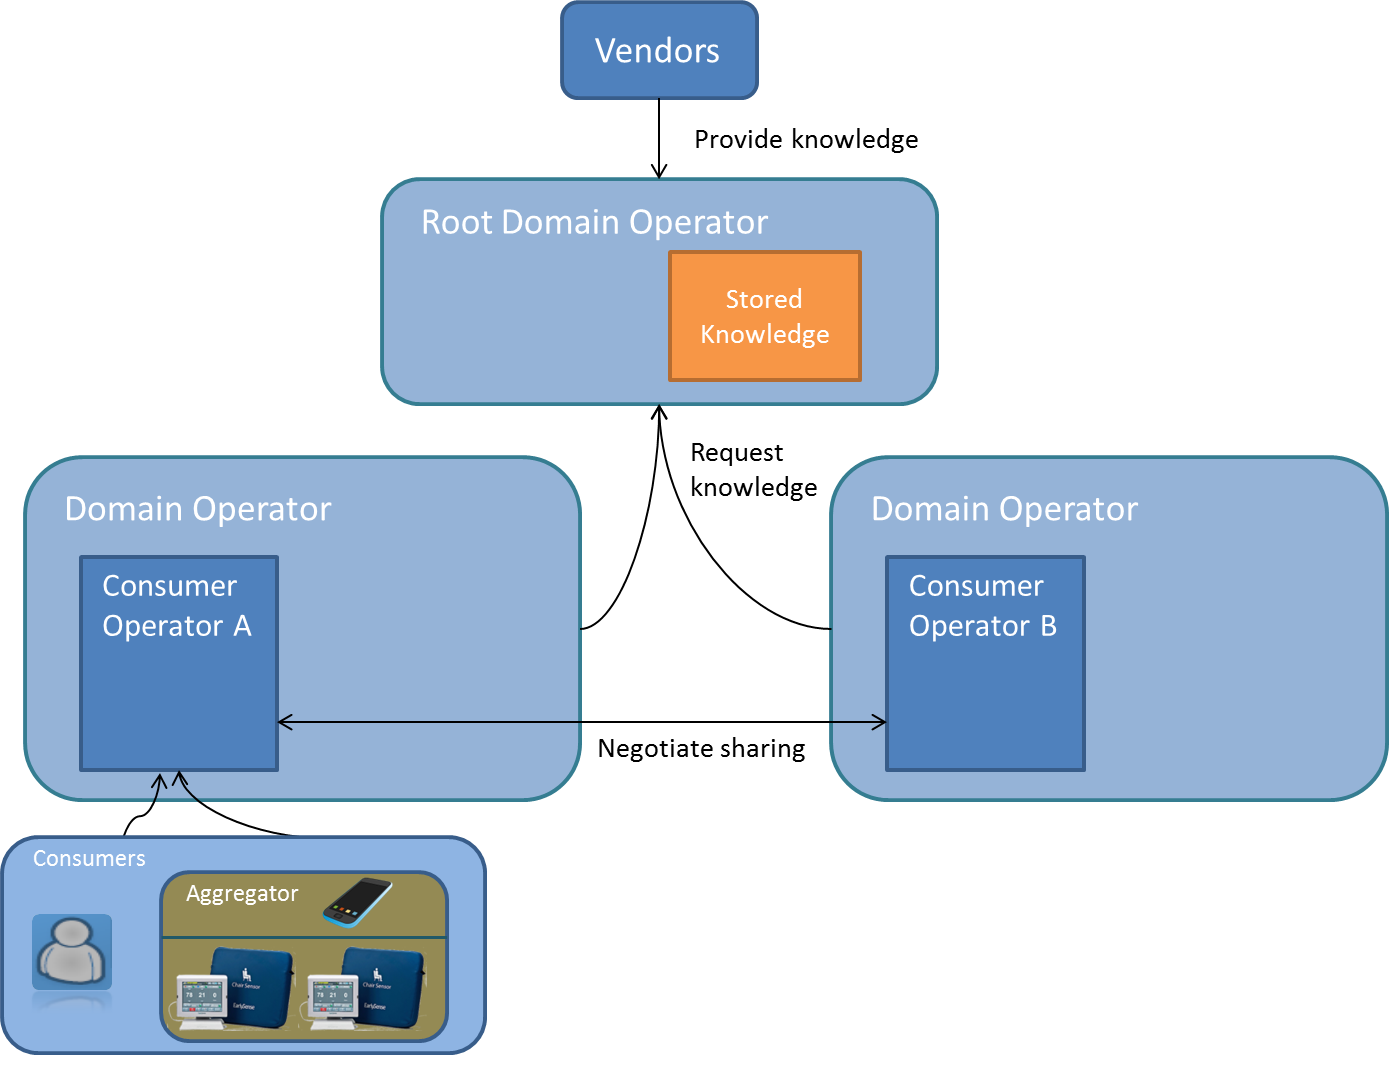
\includegraphics[width=0.8\textwidth]{images/design.png}\\
	\caption{Global architecture}
	\label{fig:concept__architecture}
\end{figure}

In this architecture, the Domain Operators take the role of Device Operator and act as service providers. The devices they operate are used within aggregators, a virtual layer (software entity) that integrates devices and which is generally situated where the devices are. Typically, a consumer's mobile phone plays the role of the Aggregator and allows the consumer to handle every device and the read the data from them. It contains thus among other the required middleware for loading the drivers and software that a device needs, and for establishing a reliable communication channel between the devices and the other actors. Since aggregators communicate with other entities, it has to be authenticated.

	Besides, the process of provisioning a device involves several steps and management services like accounting or decision making. In order to hide this complexity from the end users (i.e. Consumers), an Operator, called Consumer Operator, has been introduced. A Domain Operator can have several Consumer Operators, each handling different Consumers and devices. When a Consumer wants access to a device, it requests its Consumer Operator first.
	
	The Domain Operator provides the infrastructural and organizational capabilities (like Consumer registration) whereas the Consumer Operator provides the end services to the Consumers like selling them access to devices. The Consumer, requiring access to a protected resource, needs to be authenticated. 

It can happen that the required device is not operated within the Domain of the Consumer Operator. In this case, the Consumer Operator must first request which other Operator owns the device. Once it retrieves this information, if the two Consumer Operators are bound by a contract, the device's access can be provided. Of course, the requesting Consumer Operator must be authenticated within the Domain of the other one.

In this scenario, the Consumer Operator needs to know which other Consumer Operator handles a specific device. For this request to succeed, global knowledge has to be stored. Which device is operated by which operator for example. In the same way, it is assumed that the Operators are provided with all the knowledge which is required for operating a device. But when integrating a new unknown device, this knowledge must be first retrieved. \\Therefore, in the already defined system, two other entities have been introduced: the so-called Root Domain Operator is placed on top of the Domain Operators and stores global knowledge about devices and existing Operators; the Vendor Entity represents vendors (of devices), which are part of the global process and furnish knowledge about the different devices. Since the Vendors communicate with the Root Domain Operator about protected and required knowledge, it must also be authenticated within the Root Domain Operator. 

When the Consumer Operator retrieves which other Consumer Operator operates a specific device, it then request the Root Domain. The requesting Consumer Operator acts for the Root Domain Operator as a client requesting access to a protected resource, and must then be authenticated by the Root Domain Operator.

In the end, four entities must be authenticated: the Consumers, the Aggregators, the Operators (Consumer and Domain) and the Vendors. The entities performing authentication are the Domain Operators (Root and non-Root).

But since several Domain Operators exist at the same time, it is legitimate to specify where should which entity's record be kept. A Consumer or an Aggregator is supposed to communicate only within its Domain. A Domain Operator stores therefore information about its own consumers and aggregators. In the same way, Vendors information are only stored in the Root Domain. The Operators (Consumer and Domain) are susceptible to communicate with any other Operator. But the only Entity that knows every other Operator is the Root Domain. The Operators records are thus stored within the Root Domain, which can then share its knowledge.

The different processes among thse \emph{device cloud} involve also roles and authorization. An example for that is access revocation, which could be needed in the following E-Health application case: an emergency occurs requiring customer A to have control over device D, but customer B is using the device D at that time. The access must then be revoked before the device is re-attributed to customer A. In this case, only the Device Owner or Device Operator can take such a decision. Roles and authorization must therefore be handled.

\subsection{Variety of protocols, frameworks, technologies}
As said above, in the IoT, one remaining problem is the standardization. Each device vendors designs its own proprietary protocols and technologies. In regards to security, the same phenomenon can be observed. The way encryption is done, if it is, is one of the examples. The second example is the communication protocols. A robust security system is supposed to establish reliable channels of communication between the different actors and ensure that no harm can be done to the system. 

In the \emph{device cloud}, the devices are dynamically provisioned and thus the different devices protocols cannot be statically configured at the right location. The architecture of an authentication and authorization layer must comply to this flexibility.

Independently from the devices, authentication and authorization in distributed systems has been a rich field of research. One could rely on a Password-authenticated key agreement \cite{Hao2011}\cite{Pointcheval2012}\cite{Juang2008}, symmetric or asymmetric encryption\cite{Denning1982}, on the Diameter protocol, the kerberos protocol\cite{neuman2005kerberos}, the Otway–Rees protocol, OAuth 2.0\cite{hardt2012oauth}, openID\cite{Ghazizadeh} and openID connect \cite{sakimura2014openid}, SPX\cite{Tardo1991} or some others. A. Liebl tried in 1994 to list the possible authentication protocols, showing already in 1994 a wide range of possibilities. His list is given in appendix 1\cite{Liebl1993}.

In addition, it should be also taken into consideration that a part of the implementation will eventually run on the devices platforms. 

Within these platforms, resources are limited and computation power can be low. Hence, heavy-weight framework and protocols should be avoided.

%Regarding breaches and potential attack when it comes to distributed systems, it seems that a few possibilities stand out: a Kerberos based system, an OpenID system, or a system based on an OAuth protocol (like OpenID connect). More details will be given is chapter \ref{cha:conceptanddesign}.



%If the use of libraries is chosen, the a specific library should be elected. Talking about OpenID connect, which is quite recent, six libraries at least are available. Kerberos, a much older protocol, can be implemented from basically any existing security framework. 


\section{Aim and Objectives}
This thesis, as aforementioned, is based on a global design of a \emph{device cloud}, which has also been partially implemented. However, in this design, the existence of an authentication and authorization layer is assumed. Neither the protocols or frameworks nor the methods used are specified.

This thesis will provide such a framework for Pools of dynamically provisioned devices (the so called \emph{device cloud}). This framework will also be implemented and integrated into the already existing implementation.

The protocols (communication, encryption, etc) will be specified, as well as the methods provided by the framework. The authentication and authorization framework designed here will be based on OpenID Connect. This choice is explained further in Chapter \ref{cha:03:design_concept}. 

The implementation encompasses both a User Directory (server-side) and different client-sides. The User Directory is the main component of the authentication framework and allows among other every Domain Operator to authenticate other actors of the \emph{device cloud}. It is maintained locally by every Domain Operator for authenticating their own "users" (which can be one of the four entities described above). The User Directory used in the \emph{device cloud} should have the same implementation for every Domain Operator (in particular Root and non-Root Domain Operator), and thus should implement the required level of abstraction to be used indifferently in any Operator.

For the system to be complete, different client sides (requesting authentication, etc) should be also implemented. Those clients will for example be used by the vendors or the consumers and will communicate with the User Directory of their Operator. As said above, a client should be deployed onto limited-resources platforms (for aggregators for example) and should be thus be kept as light as possible. However, the Clients created during this thesis were used only for testing purposes, and will therefore not be presented. 

It should also be decided if the User Directory relies on a dedicated database (storing users, session information) or if it should be wrapped onto an existing IAM (Identity and Access Management) solution, as an LDAP for instance. In our case, the implementation of the authorization and authentication framework is based on a LDAP.

Since several Domain Operators exist at the same time, it is legitimate to specify where should which entity's record be kept. For example, a Consumer or an Aggregator is supposed to communicate only with its Operator. It is subsequently mandatory, that a Domain Operator stores information only about their own consumers and aggregators. In the same way, vendors information should be only stored in the Root Domain. On the contrary, the Operators (Consumer and Domain) are susceptible to communicate with any other Operator. Since one does not want every Operator to store entries for every other ones, the Operators entries should be stored within the Root Domain, which can then share its knowledge. 

The choices made in this thesis have been met accordingly to both the requirements and the security issues.

M. Mackay et Al. recently identified the major threats in a cloud-based system as\cite{Mackay2012}: 
\begin{enumerate}
	\item Hacking attacks
	\item DDoS attacks
	\item Insider attacks
	\item Equipment failures
	\item End-to-end issues
	\item Espionage
	\item Data loss or corruption
\end{enumerate}

To those threats the risks related to the physical presence of sensors like destruction or damaging(8) can be added .

As for the User Directory, the design should respond to the issues 1, 6 and 7. The DDoS attacks(2) are performed on the network, and thus cannot be prevented by the design of a single component. The same argument can be given for end-to-end issues(5). Equipment failures(4), as equipment destruction or damaging(8), are absolutely not related to the design and implementation of a User Directory. Hence, it is out of the scope of this thesis. 

Handling with insiders attacks is more about predicting and detecting than preventing, and is based on observation of patterns and users behavior that are not visible to the User Directory\cite{Schultz2002}. However, it can be ensured that an authorized participant cannot access protected information with which it could harm the system.

Hacking attacks, Espionage and Data loss or corruption can be handled through data encryption, signatures, or other security standards (handling SQL injection, XSS attacks, etc). Thus, it must be ensured that the User Directory provides a sufficient security level in regards to those issues.


\section{Outline}
After the introduction to this thesis and its global context, the reader will be introduced to the security fundamentals; different algorithms, methods and frameworks to perform secure authentication will be presented and a more detailed overview of the \emph{device cloud} will be given.

In Chapter 3, the design of the framework developed in this thesis will be explained and the different choices enlightened (before all, the choice of the OpenID Connect framework).

Sections 4 analyses the protocol elaborated in the last section and try to prove that it is a safe protocol.

Chapter 5 will illustrate how such a protocol can be implemented. Implementation choices (like the use of a LDAP) will be explained as well as the structure of the final solution.

This thesis will finally be concluded by a summary of the work realized, and will propose possible future evolution from which the \emph{device cloud} could benefit.




\chapter{Background}
\label{cha:relatedwork}

In this section, the global system known as \emph{devices cloud} will be first detailed. Afterwards, the different possible technologies that could be used in this thesis will be introduced. Finally, an overview of the different researches and studies that have been previously performed will be given.
 
\section{The Devices Cloud}
Integrating the requirements defined in the Introduction to a more detailed view of the global system, the Figure \ref{fig:design_complete} of the \emph{devices cloud} architecture . Of course, only the information relevant for this thesis is depicted.

\begin{figure}[!ht]
	\centering
	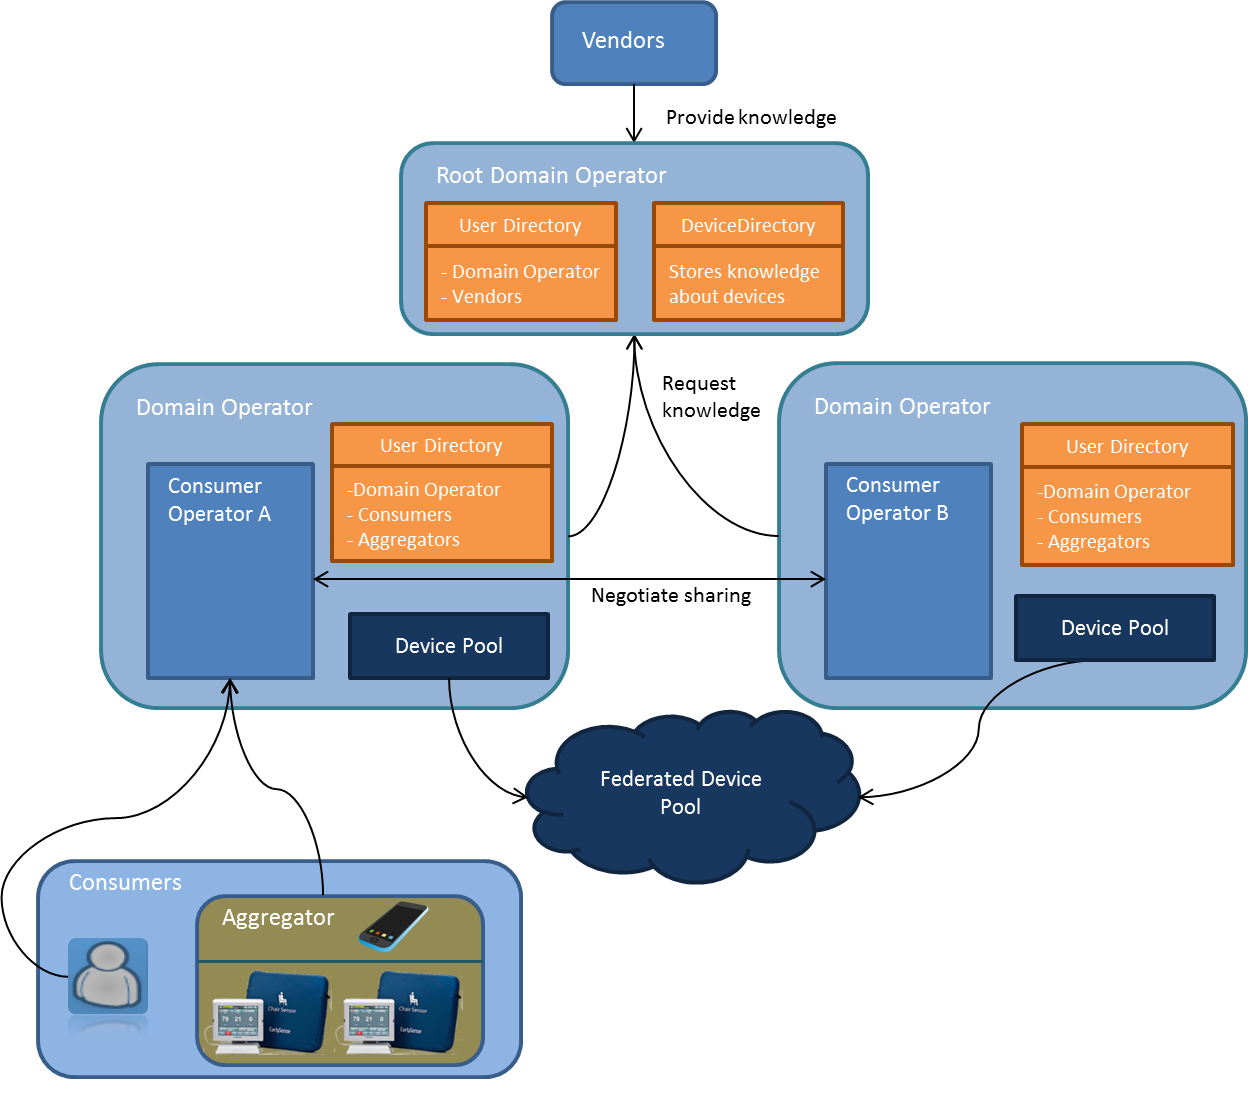
\includegraphics[scale=0.6]{images/design_complete}
	\caption{Detailed Architecture of the Devices Cloud}
	\label{fig:design_complete}
\end{figure}

\section{Authentication}
\subsection{Authentication from symmetric key}
\subsection{Authentication from asymmetric keys}
\subsection{Authentication from one-way function}
\subsection{Federated Identity Management}
\subsubsection{Kerberos}
\subsubsection{SAML}
\subsubsection{OpenId Connect}

\section{Related work}
\chapter{Concept and Design}
\label{cha:03:design_concept}

\chapterquote{In any distributed system, we are counting of the good nature of the participants to do the right thing.}{Ori Eisen, founder, chairman and chief innovation office at 41st Parameter told Sue Marquette Poremba}

Ori Eisen, meant here that as the distribution of a network becomes bigger, the harder to master it becomes. In regards to security issues, mastering is then often replaced by controlling and mitigation. 

Nevertheless, in a more restrained environment like the \emph{device cloud}, which has a top-hierarchy element - the Root Domain - higher security standards can be met. The next section explains how security and privacy are expected to be ensured in the authentication and authorization framework and describe the required infrastructural and logical architecture.

Afterwards, the methods and interfaces of the framework will be described, and a complete example will be detailed.

\section{Requirement Analysis}
It has already been explained in chapter \ref{cha:introduction} that the code would eventually be ran on devices platform, where resources are limited. Thus, heavy-weight library and frameworks are to be avoided.

The \emph{device cloud} presents another particularity. Indeed, aggregators are supposed to dynamically download the different device drivers and to execute the drivers code, also dynamically. The solution that has been chosen to respond to this need was the OGSi Alliance specification (formerly OSGi: Open Services Gateway initiative), which describes a modular system and a service platform for the Java programming language that implements a complete and dynamic component model. With this, it is possible to install, start, stop or uninstall bundles remotely and without requiring a reboot. In this context, a bundle is a group of Java classes (a jar, for example) and additional resources.

To transmit the bundles to the aggregators, the chosen solution was to use a WebSocket based approach, which uses Serialization to transfer java Objects. If the standard Serializer and Deserializer are used, the device's platform must be able to parse correctly the received Stream into any present Java class. Thus, using the default Serializer and complicated classes may demand too much resources from the devices platform and should be avoided.

Besides, most of the frameworks already existing are using the http/https schemes. OpenID Connect is originally, for example, a RESTful API. In the same way, many framework use HTTP Redirect 302 responses to redirect an End-User to the different actors. But Websocket doesn't provide default support for redirection. It must be done on the application layer. The specifications will therefore have to be adapted to the WebSocket architecture. 

Finally, as already mentioned, trust is for any distributed system a precondition for a successful functioning. In the \emph{device cloud} too, the different entities don't trust each other from the beginning. The Root Domain, in the other end, must be trusted by any other entity that communicates with him. Further on, it will be then assumed that every Domain knows how to contact the Root Domain, that it trusts the information coming from the Root Domain, and that the Root Domain will host every service that must be globally trusted (if SSL is used, the Root Domain must logically be the CA). The other trust relationships between entities will all derive from this initial trust precondition.

\section{Security Framework - Overall Concept}
\label{sec:04_framework}

The terminology used later on is partially based on the one used by existing frameworks (see \ref{02_authentication}) and partially on the \emph{device could} terminology. We thus define:
\begin{itemize}
	\item \textbf{The Principal}: a participant of the \emph{device cloud} that can be authenticated. The Principal can be a Consumer, a Vendor, an Operator (Consumer or Domain Operator), or an Aggregator.
	\item \textbf{The Client}: Client application that requires Principal authentication. They act for the Principal as service providers. In the \emph{device cloud}, client are necessarily Operators (Consumer and Domain Operators).
	\item \textbf{The Identity Provider IdP: } the entity that performs authentication of Principals for Client. Domain Operators and the Root Domain Operator are the only IdPs of the \emph{device cloud}. 
\end{itemize}

The framework defines for the Identity Provider a unique public endpoint, reachable only over a secured communication channel. This endpoint must respond to 4 different type of requests which are:

\begin{description}
	\item[\textit{Authenticate}]: A Principal is authenticated. Its information is checked, and if valid, a session is opened. The method returns the session ID of the so-opened session.
	\item[\textit{Delegated Authentication}]: A Principal is authenticated on behalf of a Client. The information of the client is checked (with this request, the Client can for example specify a return address to which the result must eventually be sent), and if valid, the user is authenticated and a proof of the Principal validity is created. This proof is returned, in form of a token, signed by the IdP.
	\item[\textit{Get Consumer profile}]: A consumer profile is asked by an Entity. If this entity is authenticated and has the corresponding rights (see section \ref{03_authorizing}), then the profile is returned.
	\item[\textit{Get Protocol URI}]: An entity wants to know how to contact a certain Operator. It requests the protocol URI defined in \ref{tab:02_entities} of this Operator. Again, the rights of the requesting entity are checked.
\end{description}

The two first requests are related to pure authentication as specified in the previous chapters. In one case, the authentication is done in a shared way, i.e. for a Client (any Operator of the \emph{device cloud}), whereas in the other case, the authentication is done in a direct way. A consumer profile can also be requested by any entity which has the right to do so.

To those three previous requests, a fourth one has been added: \textit{Get Protocol URI}. Indeed, in a distributed network, the nodes need to know how to contact their peers. Before all in a shared authentication context: If a Principal registered in an IdP A contacts a Client which doesn't know A, then the authentication cannot be achieved. The Client must be able to retrieve how to communicate with the IdP A.

In the existing applications, this is done either by statically configuring every nodes to know their neighbors, or through a dynamic services discovery process (OpenID Connect defines the OpenID Connect Discovery service, Kerberos also implement a Kerberos Discovery process, etc). In the \emph{device cloud}, one can take advantage of the hierarchical structure. The Root Domain is supposed to know every Operators within the \emph{device cloud}, so such a discovery process can be for the authentication and authorization framework be replaced by another request of type: \textit{Get Protocol URI}.

In addition to enabling Clients to retrieve the IdPs communication addresses, it also allows the IdPs to partially check the information coming from the Clients during the \textit{Delegated Authentication} process. The Clients specify an address to which the IdP's response must be sent. But since Clients are Operators, they have a ProtocolURI handled by the Root Domain. Therefore, if the return address specified by a Client is not contained by the result of a \textit{Get Protocol URI} request to the Root Domain, the Client is not considered as a valid Operator of the \emph{device cloud}.

\vspace{2em}

To respond to these requests, the IdP must implement 4 corresponding methods, listed below. It must be here noted, that the interface shows a sufficient level of abstraction for any security implementation to be used (Kerberos, OpenID Connect, ect). \textit{authenticatePrincipalForThirdParty}, for example takes as argument a Map that could contain any specific parameters. That way, the choices made further on (in the design and implementation phases) could be replaced with minimal efforts. 

\refstepcounter{foo}\label{interface_methods}

\lstset{language=Java}
\begin{lstlisting}
/**
* Authenticate a registered principal, opens a session and returns a session ticket.
*
* @param userID          the id to of the principal to authenticate
* @param secret          the secret (like password), if it has one, of the principal to authenticate. Can be null
* @param type            the principal's type, like Operator or Vendor.
* @param mode          	how the principal is supposed to be authenticated. Policies can be defined (Certificate, password, etc)
* @return a ticket, containing the opened sessionID
*/
public RequestResult authenticatePrincipal(Principalidentifier userID, EntityType type, Secret secret, AuthMode mode);

/**
* Authenticate a registered principal on behalf of a third party and returns a signed token to this party that ensure the identity and validity of the user.
*Following the receipt of this token, the third party can decide to open a session for the principal.
*
* @param issuerID       the pricipal from which the request is issued, i.e. a third party service provider
* @param extraParameters parameters added corresponding to specific security implementions (OpenID, Kerberos, ...)
* @return a token, giving proof of the validity of the authenticated principal
*/
public RequestResult authenticatePrincipalForThirdParty(Principalidentifier issuerID, Principalidentifier userID, EntityType type, Secret secret, AuthMode mode, Map<String, ? extends Serializable> extraParameters);

public RequestResult getCustomerProfile(String customerID);

public RequestResult getProtocolUris(String operatorID);
\end{lstlisting}

It is thus possible, with the methods definition above described, to utilize different security implementation, like OpenID Connect or Kerberos. The next sections will explain the choices made in regards to the authentication and authorization framework.

\section{Authentication Framework}

\subsection{Technological choice}
The basic design established so far has the sufficient level of abstraction for any security implementation to be used. However, for a more detailed description of the design, choices must be met.

The authentication and authorization framework developed here is indeed based on existing security frameworks, as presented in sections \ref{02_authentication} and \ref{02_authorization}. Obviously, a shared authentication framework is needed here, as a Single-Sign-On System, a Federated Identity Management or a trust-based system.

Considering only the age of the different frameworks, their global resiliency, and how they could fit to the \emph{device cloud} architecture (with Domains as IdP, Operators as Clients), a few stood out: Kerberos\ref{sec:02_Kerberos}, OpenID 2.0 and OpenID Connect\ref{02_OpenID}, an OAuth 2.0 based system\ref{02_OAuth}, and SAML\ref{02_SAML}.

It must be here understood, that in the \emph{device cloud}, the users identities themselves don't have to be shared. Only the authenticity of a user, i.e. if the user is authenticated within a \emph{device cloud} Identity Provider, must be shared. Hence, solutions whose FIM capability induces an important overhead or heavy dependencies should be avoided.

SAML is a widespread solution for SSO and FIM, where the different security assumptions as well as the identity characteristics of a user are shared through key-value xml-elements of the following type:

\begin{minipage}{\linewidth}

\lstset{language=XML}
\begin{lstlisting}
<saml:Assertion ID="..." IssueInstant="...">
	...								<!-- various security parameters -->
	<saml:AttributeStatement>		<!-- Defnition of a user attribute -->
		<saml:Attribute Name="the name">
			<saml:AttributeValue xsi:type="xs:anyType"> the value </saml:AttributeValue>
		<saml:Attribute>
	<saml:AttributeStatement>
<saml:Assertion>
\end{lstlisting}
\end{minipage}

Thus, if no attributes are shared, there will be no overhead induced. SAML's only drawback is that it is based on XML files. It requires complex XML signing and parsing operations that might slow some components down. Indeed, in the SAML workflow, the Principal is carrying the different messages between the Identity Provider IdP and the client RP. Those, upon receipt of a request, construct the response and redirect the Principal (normally with an HTTP 302 Redirect) and the XML files attached. But as explained above, the use of WebSocket will have the Principal parse the response and construct the XML files before sending it over. For this reason, SAML has been first ruled out.

Considering what has already been said about the need for simplicity (no heavy dependencies, etc) and this last argument, Shibboleth was also ruled out (it is based on SAML). 

Kerberos is still a major solution in authentication frameworks, is a mature framework, since it as been used for more than 2 decades, and extended resources can be found. Besides, Kerberos requires a central authority hosting both the Ticket Granting Server TGS and the Key Distribution Center KDC, and would thus easily fit to the \emph{device cloud} architecture and its Root Domain Operator. However, Kerberos shows also several significant drawbacks. First, Kerberos has strict time requirements. In the default configuration per MIT, the different clocks must have less than 5 minutes difference, which require an important synchronization effort. Secondly, it requires the Root Domain to have a great organizational and infrastructural capability. It will have to host the KDC, the TGS, and organize the PKI (certificate creation, revocation, etc). Concerning this last point, each network service which requires a different host name will need its own set of Kerberos keys. This complicates virtual hosting and clusters.

Finally, Kerberos is known to be vulnerable to password-guessing attacks. Of course, this would be a problem only if the login mode is solely based on password (that will be discussed further on section \ref{sec:03_auth_mode}) but it requires also quite a heavy configuration (hardware and software) and tend to be replaced by more recent framework in the current applications. That led to the Kerberos solution being also ruled out.

OpenID Connect and OpenID 2.0 are in fact really similar in their design. OpenID Connect is said to be the child of OpenID 2.0, an enhancement of the OpenID 2.0 features based on OAuth 2.0. As an example, in OpenID 2.0, users had to use an OpenID identifier, often quite complex, whereas in OpenID connect they can use their email. Consequently, OpenID 2.0 has been automatically ruled out for OpenID Connect. Concerning their security capabilities, J. Hodge explains that they offer very similar functionalities as SAML\cite{Hodge2008}. It is noted, that OpenID is a bit less descriptive than SAML for security issues, but as explained in chapter \ref{cha:relatedwork}, this is due to the fact that many design choices are left to the one implementing the solution. Contrary to SAML, the security assertions and identities characteristics are here based on JSON which is globally lighter and easier to process as a XML file.

Finally, one could also rely on OAuth 2.0 for the authentication and authorization framework. OAuth 2.0 is originally an authorization framework, but it could easily be turned into a way to provide authentication. This has already been done by Facebook or Google for example. However, this is exactly what OpenID connect is doing: it uses OAuth 2.0 in a secure manner (as explained beforehand, OAuth also offers a wide range of choices, which are in OpenID Connect chosen for the implementer to provide the maximum security level).

In addition, OpenID Connect is the most recent framework that has been considered here, and a lot of researches are still being conducted. Last, but not least, it is becoming a security standard, as leading IdPs (Google, Facebook) will migrate from their previous shared authentication API to APIs based on OpenID COnnect.

It has been therefore decided, that the authentication framework would be based on OpenID Connect.

\subsection{TLS-SSL, an inevitable choice}
In every secure application, the data is encrypted. It doesn't only protect the application from being hacked, it also ensure data privacy (it prevents any form of eavesdropping), which was one the concern presented in the introduction. Reviewing the specification of the main authentication frameworks presented above, all require or recommend the usage of encryption.

In the OpenID Connect Documentation, the use of the https scheme is sometimes required, sometimes recommended. In the framework, messages will then be transfered over the wss scheme, i.e. WebSocket over TLS/SSL, for every communication. All incoming connection over an insecure channel must be terminated.

The use of TLS is perfectly adapted to the architecture of the \emph{device cloud}. The Root Domain will create, deliver, and revoke the certificates of the different entities and act as the only valid Certificate Authority of the \emph{device cloud}.

\subsection{Authentication mode}
\label{sec:03_auth_mode}

The authentication of a principal relies on its capability to prove its validity and authenticity to its Domain Operator. This can be done by a shared knowledge between the principal and the Domain Operator (Proof by knowledge), by the possession of an object that only the principal is supposed to have (Proof by possession), or by something that the user is or does (Proof by property).

Some of the principals to authenticate, namely the operators and the aggregators, aren't human beings. This makes it far more complicated to set up an authentication method with proof by knowledge. Besides, proof by knowledge is often weak in itself, because the knowledge chosen by the users, if too simple, is easy to guess.

In the same way, proof by property is hard to achieve with non-human entities. One cannot use DNA comparison, iris or fingerprint recognition. Anyway, in the context the \emph{device cloud}, which is a cloud service, it appears to be not flexible enough.

The best way to authenticate the principals is therefore the proof by possession. Based on the architecture already defined, an obvious choice stands out. Indeed, the use of TLS/SSL enables the so-called SSL Certificate authentication. As explained in the introduction, TLS/SSL originally only authenticate the server to the Principal, but if both entities have a certificate signed by a Certificate Authority, mutual authentication can be performed. It doesn't mean that the server knows directly which Principal it is communicating with, but only that this Principal is a valid entity of the \emph{device cloud}, since it has a valid certificate.

To perform a true authentication, the server can then extract the Principal identifier from the certificate. This has been the solution chosen for the authentication framework. It is supposed that the Root Domain will deliver signed certificates to the different entities, containing among other the entities IDs.

How those certificates are effectively created, delivered, or revoked is out of the scope of this thesis. It is ensured though, that the certificates can be delivered in a secure way without compromising any critical information in the process. For example, the creation of an Principal account could be the result of a request over a TLS/SSL connection. This SSL connection wouldn't be configured to require mutual authentication, but only server authentication. Any data transfered after the SSL handshake will be then only understood by the correct actors (Principal and IdP). The final step could then be the transmission of the certificate to the Principal.

Finally, even if SSL certificate authentication is the default authentication mode in the framework, one still can add other proofs to validate the identity of a Principal. Subsequently, it has been decided to let the possibility to specify an additional type of proof, like password for example. This could be set up to enhance the security for human entities as the Consumers, and can be customized by every Domain.

\subsection{Principal Persistence}

As evoked earlier, persisting Principals within a Domain can be done either with a dedicated database, or with an existing IAM solution.The Domain Operator will create new Principals and verify the validity of incoming connections with this persistence system.

The framework let the Domains decide which persistence solution they want to implement. Nonetheless, several properties are specified:

\label{LDAP_security}
\begin{itemize}
	\item The communication channel with the persistence system must be secured with TLS/SSL
	\item The Domain Operator must be the only entity with access to the persistence system, i.e. only one user has the privileges to modify and read the data
	\item As a subset of the measures that one can met for the previous requirement, Host filtering should be enabled to prevent anyone else to even connect to the persistence system. However, enabling it will never be a sufficient condition. A program running on the same host as the User Directory but with other privileges could access the LDAP, or if NAT (Network address translation) is used, any host sharing the same external IP also could.
	\item The persistence of Principals and the persistence of any other data should be kept separated into two different systems. This permits to reduce the surface attack that a hacker can have on the persistence system.
\end{itemize}

\section{Authorization Framework}
\label{03_authorizing}

\subsection{Access Control Model}

In the \emph{device cloud}, there exist several actions for which access control must be performed. This access control involves among other the roles defined in chapter \ref{cha:introduction}: EntityOwner and EntityOperator.

The framework proposed here defines a dynamic access control matrix $ M_{t}:  P_{t} \times O_{t} \rightarrow 2^{R}$ where $P_{t}$ are the set of principals,  $O_{t}$ the entities handled in the framework and R the set of possible actions. A simple access rule can be then formulated as: "a principal $p \in P_{t}$ can do $r \in R_{t}$ with $o \in O_{t}$".

As defined in the chapter \ref{cha:relatedwork} a principal $p \in P_{t}$ can be an Aggregator, Vendor, Consumer or Operators, whereas an entity $o \in O_{t}$ can be a principal itself, consumer profile or a ProtocolURI, as explained in section \ref{sec:04_framework}. The ProtocolURI, will be however treated as a subpart of the entities, since it is an attribute of Operators. 

The following set of actions is defined:
\begin{itemize}
	\item \textit{Read-Only} - read access to an entity
	\item \textit{Read-Write} - read and write access to an entity
	\item \textit{Create} - permission to create an entity of a particular type
	\item \textit{Delete} - permission to delete an entity
\end{itemize} 

\vspace{0.5em}
The table \ref{tab:access_control} lists the different actions and the corresponding rights. The only one that can access the Principals entities for any action is the EntityOperator. In the \emph{device cloud}, this is the Domain Operator in which the Principals are subscribed.

Regarding the Consumer Profile, the only one that can create, remove or update (Read-Write access) is quite logically the Consumer owning the profile. However, its profile must be readable for the entities that manage the Consumer or can interact with him. For this reason, two groups of users have been added to the ones allowed to read the profile. In the first place, the EntityOperator of the profile, and in the second place, a group of users defined by the Consumer itself.

 %	 \setlength{\extrarowheight}{15pt}
 \begin{table}[htpb]
 	\caption{Actions, Entities and Rights} 
 	\label{tab:access_control}
 	\begin{tabular}{|m{0.9\textwidth/50*8}|m{0.9\textwidth/50*12}|m{0.9\textwidth/5}|m{0.9\textwidth/5}|m{0.9\textwidth/5}|}
 		\hline
 		\cellcolor{Gray} & \multicolumn{4}{c}{\cellcolor{Gray}\textcolor{white}{\textbf{Actions}}}\\
 		\hline
 		\cellcolor{Gray}\textcolor{white}{\textbf{Entity}} 
 		&
 		\cellcolor{LightGray}{Read-Only}
 		&
 		\cellcolor{LightGray}{Read-Write}
 		&
 		\cellcolor{LightGray}{Create}
 		&
 		\cellcolor{LightGray}{Delete}
 		\\ \hline
 		
 		\cellcolor{LightGray}principal & \textbullet \quad EntityOperator. \linebreak \linebreak \textbullet \quad For the property protocolURI of the operators: every operator (see section \ref{sec:04_framework}) & EntityOwner & EntityOwner & EntityOwner
 		\\ \hline
 		\multirow{3}{*}{\cellcolor{LightGray}} & 
 		\multicolumn{1}{p{0.8\textwidth/9*2}|}{\textbullet \quad EntityOwner (the consumer linked to the profile)} & 
 		\multicolumn{1}{p{0.8\textwidth/9*2}|}{EntityOwner} &
 		\multicolumn{1}{p{0.8\textwidth/9*2}|}{EntityOwner} & 
 		\multicolumn{1}{p{0.8\textwidth/9*2}|}{EntityOwner} 
 		\\
 		\cellcolor{LightGray}consumer profile & 
 		\textbullet \quad EntityOperator & 
 		& 
 		& 
 		
 		\\
 		\cellcolor{LightGray} & 
 		\textbullet \quad A set of allowed users defined by the Consumer owning the profile &
 		& 
 		& 
 		
 		\\

 		\hline
 	\end{tabular}
 \end{table}


\subsection{Authorizing}
\label{03_consumer_profile_authorization}
Several choices were possible to perform authorization within the \emph{device cloud}.

Since it was decided to use OpenID Connect for authentication, the framework for authentication and authorization would already support OAuth 2.0. It seemed then quite natural to use a shared Authorization framework as OAuth 2.0. Using the terminology of OAUTH 2.0 presented in section \ref{02_OAuth}, the flow of authorization would be, for the Consumer Profile, as follows:

\begin{enumerate}
	\item The Client RP (like a Consumer Operator) asks the Authorization Server a consumer profile.
	\item The Authorization Server asks the Consumer if it allows the Client to access its profile.
	\item A Grant Token is returned to the Client.
	\item The client authenticates to the Authorization Server and exchanges its Grant Token against an Access Token.
	\item The Client requests the consumer profile from the Resource Server using its Access Token.
\end{enumerate}

This approach has two main drawbacks. Indeed, it requires the consumer to express its consent every time another entity wants to access its profile. This might work well in the www word, because the user is connected by the time it is asked for its consent (when a service wants to access the facebook profiles photos for example), but in the \emph{device cloud}, since devices are provisioned dynamically, an entity could want to check a consumer profile at any time.

The second drawback comes from the fact that access control rights are defined statically in the \emph{device cloud}. As explained above, a consumer can indeed define a set of allowed users. This works here because the consumer knows a-priori the entities that must be allowed. On the contrary, the OAuth 2.0 solution is more intended to be used when the consumer doesn't know the different service providers beforehand.

The chosen solution was therefore to use a static access control management, where entities like the Consumer profiles are persisted with their authorization attributes, like a group of allowed users or an EntityOperator, etc.

\subsection{Entities and their authorization properties persistence}
\label{sec:03_database}
As explained above, any data which is not an Principal should be persisted in a different persistence system than the one used for authentication (for principals).

This way, if the persistence system discussed here is compromised, the data related to the Principals and their secrets (passwords, etc) won't be disclosed.

The consumer profiles and their properties could then be persisted in a simple SQL database for example. However, the persistence system that is used for the data must be secured, exactly like the system used for principals.

The following requirements are specified:

\begin{itemize}
	\item The Domain Operator must be the only entity with access to the persistence system, i.e. only one user has the privileges to modify and read the data
	\item Host filtering should be enabled to prevent anyone else to even connect to the persistence system
	\item The communication channel with the persistence system might be secured with TLS/SSL
	\item Private and sensitive data like the various sets of allowed users might be encrypted. The encryption process used is not specified
\end{itemize}

One really secure way of providing secure communication channels and encrypted data would be to always use TLS/SSL for communicating with the database, and put the database on an encrypted hard drive. Of course, extra security measures have to be met for ensuring that the decryption key can't be easily disclosed.
	


\section{An example}
Let's consider a complex case in the \emph{device cloud} and apply the design to it.

Most of the time, Principals like Consumers or Aggregators will stay within their Domain. However, in case where a consumer wants a device that is not operated by its Domain, the requests can span domains.

Let's then consider the Consumer C, its Consumer Operator CO1, their Domain Operator DO, the Root Domain RD, and the remote Consumer Operator which operates the required device, CO2.

The process of provisioning the device, depicted in fig\ref{fig:example}, would follow the next steps:
\begin{enumerate}
	\item The Consumer C contacts its Consumer Operator CO1 and asks for a device. CO1 doesn't know C, and thus begin a delegated authentication request with its Domain Operator DO. 
	\item The delegated authentication process takes place. CO1 redirects C to the Identity Provider DO, where C is authenticated (Additional steps for authentication might occur here). Eventually, C is redirected to CO1 with a proof of its validity.
	\item CO1 can now open a session for C and handle the initial request. It checks whether it operates the requested device. Since it doesn't, it retrieves the Operator that does, CO2 (the EntityOperator of the device) and asks the root Domain RD for the protocolURI of CO2. For that, it authenticates before to RD. 
	\item Once it has the protocolURI, CO1 can requests the device from CO2.
	\item CO2 doesn't know CO1. Again, a delegated authentication request is initiated, with the Root Domain RD as IdP.
	\item Once CO1 is authenticated, CO2 can provision the device to CO1, which in turn re-provision to its Consumer C.
\end{enumerate}

\begin{figure}[!ht]
	\centering
	\subfloat[delegate authentication process][Step 2 \& 5: delegate authentication process. Step 2 presented.]{
		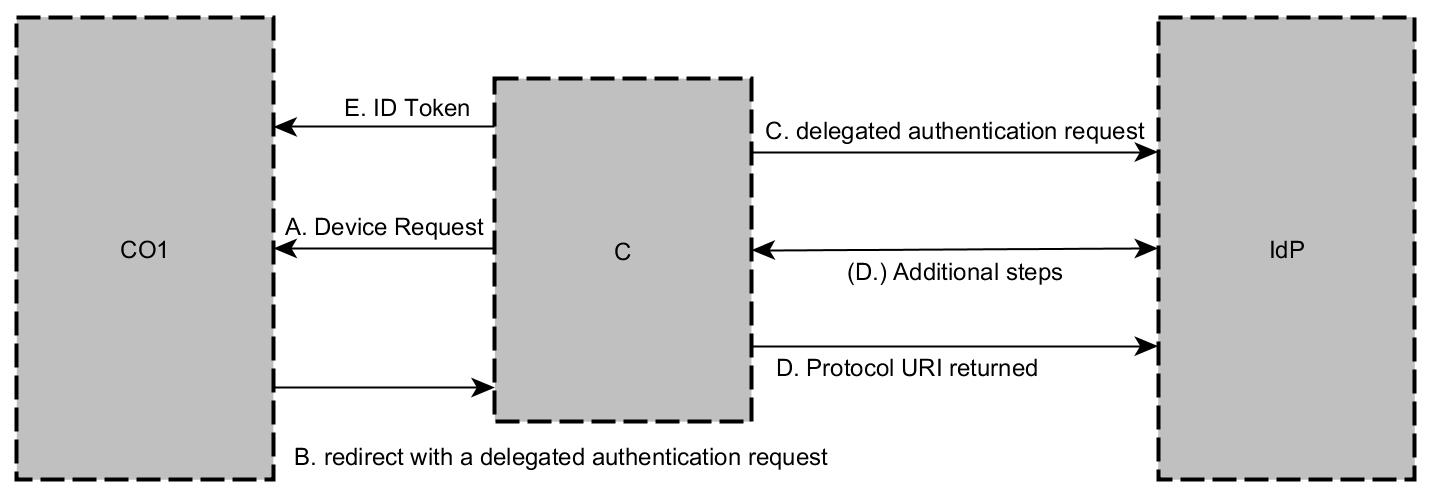
\includegraphics[width=\textwidth]{images/case1}
		\label{fig:example_a}}
	\qquad
	\subfloat[authenticate \& get protocol URI processes][Step 3: authenticate \& get protocol URI processes]{
		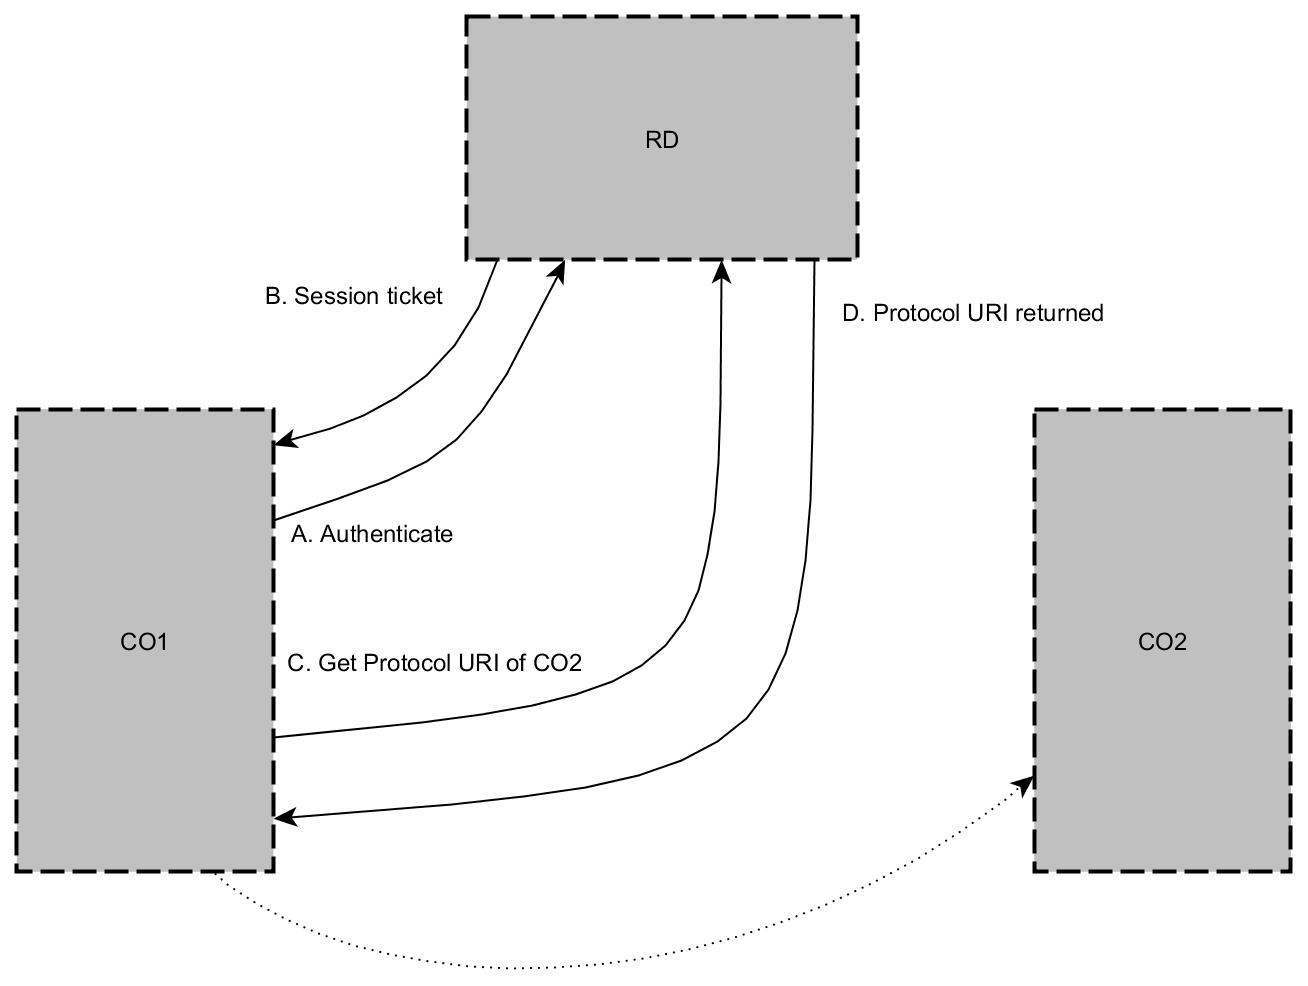
\includegraphics[width=\textwidth]{images/case1_b}
		\label{fig:example_b}}
	\caption{Main steps in the provision of a device crossing domains.}
	\label{fig:example}
\end{figure}

\vspace{1em}
In the process, the only two assumptions made are that every entities trusts the Root Domain (any communication is done over a secure channel, where entities certificates must be validated by the Root Domain certificate) and that the various Operators know how to contact the Root Domain Operator. From those two assumptions, it will later on proved that the design is secure, or at least robust (the zero-risk level doesn't exist in security)\ref{cha:evaluation}.

The possibility to add additional step when authenticating a Principal is also given, as shown in Fig \ref{fig:example_a}. For instance, the IdP could ask the Principal to sign a message with another key. Even sophisticated features like One-Time Passwords (a Consumer would receive a one time code by SMS) could be considered. 

Also, it is assumed that the Principal can send its credentials when redirected from the Client to the IdP. In a normal http environment, the Principal only conveys the message when redirected, but since Websocket redirection are handled on the application layer, this would not be a problem. However, if a Principal forgets to attach the required data, the IdP can request it, thus leading to additional steps.



\chapter{Evaluation}
\label{cha:evaluation}

The evaluation of the thesis should be described in this chapter
\chapter{Implementation}
\label{cha:implementation}

Describe the details of the actual implementation here...
\chapter{Conclusion}
\label{cha:conclusion}

This thesis presented and evaluated an authentication and authorization framework for  Pools of dynamically provisioned devices. This chapter concludes the thesis with a summary of the achieved work and gives as well a few leads for possible future works.

\section{Overview of the thesis}
The main goal of this thesis was to design a secure global authentication and authorization framework for environments where devices are dynamically shared, like the so-called \emph{device cloud}. The design mainly focused on the security aspects, on one hand, and on the other hand on the specificities of such an environment. The different entities (the ones that can be authenticated, the Principals, the ones that can perform authentication, the Identity Providers, or the ones that just require the Principal authentication without directly performing it), how those entities are structured (a hierarchical structure with a root element) or technical specificities (potentially limited resources platforms, the use of Java Serialization). 

Several existing frameworks or protocols, on which the solution could have been based on, were considered. The final call was to use a SSL Certificate authentication for a direct authentication, with the possibility to add extra authentication methods (like password or One-Time-Password) and to extend the OpenID Connect specification for performing authentication for a Client.

Concerning the authorization issue, a static process was chosen: every entity is persisted with attributes like EntityOwner(which represents the owner of the entity) or EntityOperator, on which the authorization to create, read, update or remove the entity is based. A Consumer can for example define a group of users who are allowed to read its own Consumer Profile.

Afterwards, the design was evaluated in terms of resiliency, i.e. could one find potential flaws in the framework. For this purpose, the framework has been first logically modeled, then analyzed by an automated procedure. With all three different flaws detection algorithms used, no breaches could be found. The framework designed in this thesis can therefore be deemed as secure.

As a final step, the main component of the framework, an Identity Provider, as well as a few Clients, were implemented and tested. It was done in such a way, that every Identity Provider of the global system could have the same implementation. The way they perform authentication, though, is customizable. In this thesis, a LDAP was chosen with the possibility to add a password in addition to the certificate authentication.

\section{Future research}

This sections describes possible direct extensions of the work presented in this thesis, as well as leads for future research.

\subsection*{A more detailed evaluation}
\addtocounter{subsection}{1}
The evaluation proposed in this thesis relies on an automated tool, namely the AVISPA tool. The protocol has been evaluated as secure, but one of the algorithms used for flaws detection (the OMFC algorithm) has not been updated since 2006. 

Other tools for detection could be tried, like the Automated Validation of Trust and Security of Service-oriented ARchitecture (AVANTSSAR) project, which was quite successful since it for example helped discover flaws in the Google SAML protocol. 

An other approach could also be tried, like attempting to logically prove that the framework is secure. For that a logic like the BAN logic, but which would fit the shared authentication infrastructure, should be first found.

Finally, the thesis also aimed at minimizing computational and memory cost for End-Users, since their implementation might be deployed on limited resources platforms. For now, the only evaluation in regards to this concern is that the extra dependencies added by this thesis represent about 2 Mbs, which is little. Nevertheless, this might not be sufficient to assess the good functioning of the solution proposed here. Therefore, a test in real conditions or at least in a realistic simulated environment should be performed.

\subsection*{Accountability}
\addtocounter{subsection}{1}

The idea of a \emph{device cloud}, a pool of dynamically provisioned devices, can be interesting for an industrial actor but only if seconded by a good billing system. 

	In this context, accountability becomes a matter of first importance. It provides the required capabilities for tracking the activity of an End-User, determining the duration of a session or which services / resources have been accessed. Of course, such processes rely heavily on the authentication process.

Hence, it is a logical follow-up of this thesis. In the \emph{device cloud}, accountability is still an open issue. The following list is an example of several questions that should be answered, : 
\begin{itemize}
	\item Who can perform accountability ? Domains, or Operators (Consumer Operator, Domain Operators, both, etc).
	\item For who is it performed ? (there are different types of End-Users).
	\item What can be measured, how and when ? (as already seen, the process of provisioning a device can involve quite a lot of actors. At which point of the process is which information saved). 
	\item How reliable are the accountability processes ?  (If an End-User requests a device, it should first download the drivers and install them. Can this time, during which it is not using the device, 	be estimated ?).
\end{itemize}


\subsection*{Integration}
\addtocounter{subsection}{1}
In \citetitle{reference_thesis}, the implementation of \emph{device cloud} basis is already described. But since the authentication and authorization framework was an assumption, anyone could basically access any resource or authenticate. Now that the framework has been designed and implemented, it is possible to simulate the \emph{device cloud} in its entirety. 

It would be the occasion to finally simulate the hierarchical structure, and to perform real conditions tests.




%--------------------------------------------------------------
\backmatter

\listoftables
\listoffigures

\setwidesite{}						% Set page to be wider for bibliography

\label{cha:bibliography}
\markboth{Bibliography}{Bibliography}
\addcontentsline{toc}{chapter}{Bibliography}
\printbibliography
%\printbibliography[heading=offline,filter=offline]
%\printbibliography[heading=online,filter=online]

\begin{appendices}

\chapter{Appendix 1}
\label{appendix:listing1}

\lstset{language=PHP}
\begin{lstlisting}
for($i=1; $i<123; $i++)
{
    echo "work harder! ;)";
}
\end{lstlisting}
\chapter{Appendix2: Kerberos}
\label{appendix:kerberos}
This appendix describes in detail the Kerberos authentication flow. This flow is depicted in Figure \ref{fig:kerberos}.

\begin{figure}[!ht]
	\centering
	\caption{Kerberos authentication flow}
	\label{fig:kerberos}
	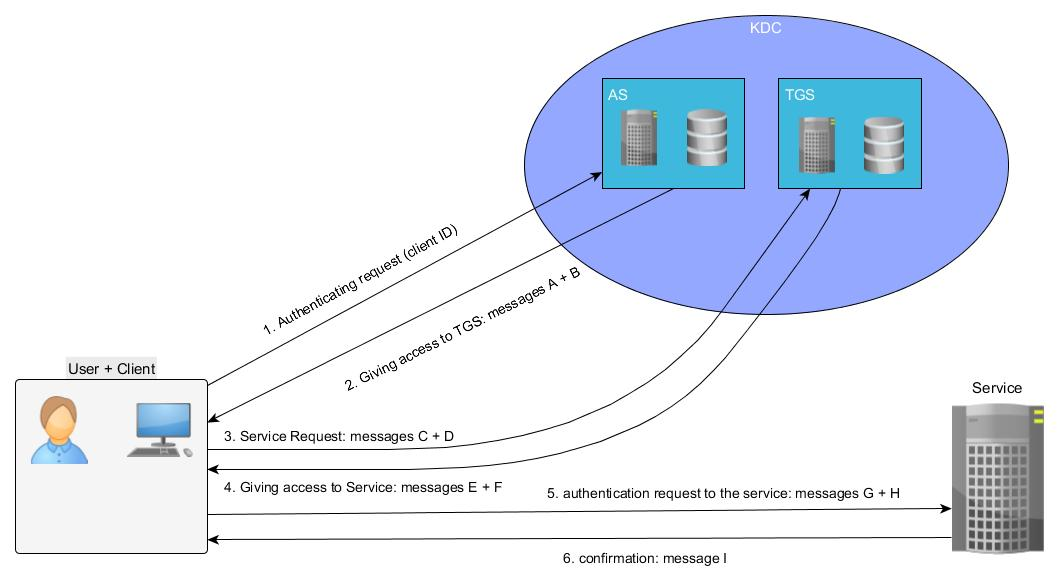
\includegraphics[scale=0.4]{images/kerberos}
\end{figure}

\begin{enumerate}
	\item The user first authenticate with the Authentication Server. This step consists only in sending the user ID in clear text (it is assumed that the user is already registered, and that the AS knows the keys of all its users).
	\item The AS checks if it knows the user. If yes, it sends two messages back: 
	\begin{enumerate}[label=\bfseries\Alph*)]
		\item client TGS session key $k_{TGS/user}$ encrypted with $k_{user}$;
		\item $TGT$ (Ticket Granting Ticket), which allows the client to contact the TGS. It contains the predefined TGS session key  $k_{TGS/user}$, along with the client ID, the client network address, the validity time of the ticket, etc. The $TGT$ is encrypted with $k_{TGS}$ so that only the TGS can decrypt it.
	\end{enumerate}
	The client can decrypt A but not B, since it doesn't know $k_{TGS}$. From what it now has, the client can request services access.
	
	\item The client requests a specific service, by sending the two following messages:
	\begin{enumerate}[label=\bfseries\Alph*), resume]
		\item $\lbrace TGT, service ID \rbrace$
		\item $Authenticator=\lbrace client ID, timestamp \rbrace$ encrypted with $k_{TGS/user}$ 
	\end{enumerate}
	Once again, only the TGS can decrypt both of the messages.
	
	\item When receiving message \textbf{C} and \textbf{D}, the TGS verify that the ticket $TGT$ is valid and decrypt the $Authenticator$ with the session key of the user. It is assumed here that every services are formerly registered to the TGS, so that the TGS has the key of the required service. If it has it, it then sends the two following messages:
	\begin{enumerate}[label=\bfseries\Alph*), resume]
		\item Client / SS session key $k_{SS/user}$ encrypted with $k_{TGS/user}$.
		\item Client to AS Ticket, containing information aimed at the server ($k_{SS/user}$, validity period, user ID, user address, etc). It is encrypted with $k_{SS}$ so that only the Service Server can decrypt it.
	\end{enumerate}
	
	\item The client know has enough information to connect to the SS, with the two following messages:
	\begin{enumerate}[label=\bfseries\Alph*), resume]
		\item same as H.
		\item New $Authenticator$ containing the client ID, a new timestamp, encrypted with $k_{SS/user}$.
	\end{enumerate}
	
	\item When the Service Server receives both messages, it can decrypt the session key, and confirm its true identity with a last message
	\begin{enumerate}[label=\bfseries\Alph*), resume]
		\item The timestamp found in message H + 1, encrypted with the session key.
	\end{enumerate}
\end{enumerate}
\chapter{HLPLS logic}
\label{appendix:hlpls}

\section{direct authentication}

	\lstset{language=HLPSL}
	\begin{lstlisting}
	% ***********************************************************
	% *   The user Party role of the OpenID Connect protocol    *
	% ***********************************************************
	role user(U, R : agent, 		%the End-User Agent, a client third-party, and an IdP Provider (an Operator)
	RCV_RU, SND_RU : channel(dy),
	Ku: public_key,		% the public key of the user, used in its SSL certificate
	Kca: public_key, 	% SSL certificate authority
	Kru: symmetric_key, % imitate SSL between end-user and the other parties
	Certificate: message,
	ResourceID: nat)	% the id of the protected resource to request
	played_by U	def=
	local State : nat, 		% internal state 
	CACertificate : message,
	Kcertificate : public_key,
	AgentCertificate : agent,
	Nb : text, 		%nonce for auth simulation
	Secret, SignedNonce : message,		% protected resource
	SessionID: nat
	init State := 0
	transition
	% 1. first transition, send certificate:
	1. State = 0 /\ RCV_RU(start) =|>
	State' := 2 /\ SND_RU({U.R.Certificate}_Kru)
	% 2. Receives Nonce from the server for mutual authentication: decrypts with the public key of the IdP and sends it back signed with its own private key.
	% Receives also the IdP certificate signed by the CA.
	2. State = 2 /\ RCV_RU({SignedNonce'.{AgentCertificate'.Kcertificate'}_inv(Kca)}_Kru) /\ 
	SignedNonce' = {Nb'}_inv(Kcertificate') =|>
	% authenticate and ask for a protected resource
	State' := 4 /\ SND_RU({{Nb'}_inv(Ku)}_Kru) /\ witness(U,R,op_user_authentication, Nb')
	% Receives "ok" and request resource
	3. State = 4 /\ RCV_RU({SessionID'}_Kru)  =|>
	State' := 6 /\ SND_RU({U.R.ResourceID.SessionID}_Kru)
	% 3. Asks for private resource
	4. State = 6 /\ RCV_RU({Secret'}_Kru) =|>
	State' := 8
	end role
	
	
	% ***********************************************************
	% *    The IdP Party role of the OpenID Connect protocol    *
	% ***********************************************************	
	role idp(R : agent, 
	SND_UR, RCV_UR : channel(dy),
	Kroot: public_key,
	Kca: public_key,
	Kru: symmetric_key,
	ProtectedResource: message,
	ResourceIDs: nat set,
	CACertificate: message)
	played_by R	def=
	local State : nat,
	U : agent, 		% the requesting client, and a aser to authenticate
	Nb : text, 		% for auth simulation
	Kcert : public_key, 	% public key used by any party
	ResourceID, SessionID: nat,
	Sessions: (nat.agent) set
	init State := 1 /\ Sessions := {}
	transition
	% first transition:
	% authentication request (with the certificate of the user)
	1. State = 1 /\ RCV_UR({U'.R.{U'.Kcert'}_inv(Kca)}_Kru) 
	% sends its own certificate and perform mutual authentication: sends nonce signed with the IdP's private key
	% Expect the same nonce signed with the private key of the user
	=|> State' := 3 /\ Nb' := new() /\ SND_UR({{Nb'}_inv(Kroot).CACertificate}_Kru)
	%First transition, 2nd possibility: request a protected resource
	2. State = 1 /\ RCV_UR({U'.R.ResourceID'.SessionID'}_Kru) /\ in(SessionID'.U', Sessions) /\ in(ResourceID', ResourceIDs) =|>
	State' := 5 /\ SND_UR({ProtectedResource}_Kru) /\ secret(ProtectedResource, test, {U,R})
	% Receive the signature and the request for a protected resource
	3. State = 3 /\ RCV_UR({{Nb}_inv(Kcert)}_Kru)  =|>
	State' := 1 /\ request(R, U, op_user_authentication, Nb) /\  SessionID' := new() /\ 
	Sessions' := cons(SessionID'.U, Sessions) /\  SND_UR({SessionID'}_Kru)
	end role
	
	%The session role binds the different parts of the OpenID protocol together
	role session(R, U : agent,
	Kroo : symmetric_key,
	Kca, Kroot, Kca_idp, Ko : public_key,
	Resource: message,
	ResourceID: nat)
	def=
	local SND_UR, RCV_UR,	
	SND_CU, SND_RU, RCV_CU, RCV_RU,
	SND_RC, RCV_RC : channel(dy),
	ResourcesMapping: nat -> message,
	ResourceIDs: nat set
	init ResourceIDs := {ResourceID}
	
	composition
	%The different roles bound together.
	user(U, R, SND_RU, RCV_RU, Ko, Kca, Kroo,{U.Ko}_inv(Kca), resourceID)
	/\ idp(R, SND_UR, RCV_UR, Kroot, Kca, Kroo, Resource, ResourceIDs, {R.Kroot}_inv(Kca_idp))
	end role
	
	role environment()
	def=
	const u,r : agent,
	op_user_authentication, test : protocol_id,
	kru, kiro, koi, kri : symmetric_key,
	resourceID: nat,
	protectedResource: message,
	kca, ku, ki_o, kca_fake, kidp : public_key
	intruder_knowledge = {u,r,kca,ku,ki_o,i, resourceID}
	composition
	session(r, u, kru, kca, kidp, kca, ku, protectedResource, resourceID)
	/\ session(r, i, kri, kca, kidp, kca, ki_o, protectedResource, resourceID)
	/\ session(i, u, kri, kca, kidp, kca_fake, ku, protectedResource, resourceID)
	end role
	
	goal
	% The authentication goal of the OpenID protocol - user to IdP
	authentication_on op_user_authentication
	secrecy_of test
	end goal
	
	environment()
	\end{lstlisting}
	
\section{delegated authentication}


	\lstset{language=HLPSL}
	\begin{lstlisting}
% ***********************************************************
% *   The user Party role of the OpenID Connect protocol    *
% ***********************************************************
role user(U, C, R : agent, 		%the End-User Agent, a client third-party, and an IdP Provider (an Operator)
SND_RU, SND_CU, RCV_RU, RCV_CU : channel(dy),
Ku: public_key,		% the public key of the user, used in its SSL certificate
Kca: public_key, 	% SSL certificate authority
Kru,Kcu: symmetric_key, % imitate SSL between end-user and the other parties
Certificate: message)	% the certificate provided by the CA
played_by U	def=
local State : nat, 		% internal state 
X : nat,		% unknown message of type int (simulaton of redirectURI)
Y,CACertificate, SignedNonce : message,		% unknown message (token returned by the IdP)
Na : text, 		% The nonce variable in the OpenID protocol.
Nb : text,	%nonce for auth simulation
Kcertificate: public_key
init State := 0
transition
% first transition, send dummy message that initiates the delegated authentication process:
1. State = 0 /\ RCV_CU(start) =|>
% Contact the relying party
State' := 2 /\ SND_CU({U.X}_Kcu)
% Receive redirect from the client, send it to the OpenID provider with 
% authentication information included (certificate)
2. State = 2 /\ RCV_CU({U.C.R.X'.Na'}_Kcu)  =|>
% Send the redirect message to the OpenID provider with 
% public authentication information included
State' := 4 /\ SND_RU({R.U.C.Na'.X'.Certificate}_Kru) 
% Additional step for auth - the End-User verify that the IdP is trustworthy. It receives a 
% certificate and a signed Nonce (with the private key corresponding to the certificate).
% It then proves that he has the private key related to the its own certificate.
3. State = 4 /\ RCV_RU({SignedNonce'.{R.Kcertificate'}_inv(Kca)}_Kru) /\
SignedNonce' = {Nb'}_inv(Kcertificate') =|> 
State' := 6 /\ SND_RU({{Nb'}_inv(Ku)}_Kru) /\ witness(U,R,op_user_authentication, Nb')
% Receive redirect from the IdP and send the redirect information to the Relying Party
4. State = 6 /\ RCV_RU({U.R.C.Na'.CACertificate'.Y'}_Kru) =|>
State' := 8 /\ SND_CU({U.R.C.Na'.CACertificate'.Y'}_Kcu) /\
witness(U, C, authenticate_user, {U.R.C.Na}_Kcu)
end role

% ***********************************************************
% *  The client Party role of the OpenID Connect protocol   *
% ***********************************************************	
role client(C, R : agent, 		% The client and the IdP (here, root domain) agent
SND_RC, RCV_RC : channel(dy),
Kc, Kca: public_key, 	% public keys of the client and CA
Kcr: symmetric_key,	% imitate SSL with the IdP
Certificate: message,	% certificate provided by the CA
RedirectionURI: nat)	% simulate redirectURI with Integer
played_by C	def=
local State : nat ,
U : agent, %the user wanting access to the third party
Na : text, % The nonce variable in the OpenID protocol.
Kcert : public_key, %public key used by any party
X: nat,
SignedToken: message
init State := 1
transition
% first transition: message requiring authentication from the user
1. State = 1 /\ RCV_RC({U'.X}_Kcr) =|>
%redirect with auth request
State' := 3 /\ 
SND_RC({U'.C.R.RedirectionURI.Na}_Kcr)
% Receives the positive assertion message from the OpenID provider 
% redirected from the user
2. State = 3 /\ RCV_RC({U.R.C.Na.{R.Kcert'}_inv(Kca).SignedToken'}_Kcr) /\
SignedToken' = {U.R.C.Na}_inv(Kcert') =|>
State' := 5 /\	request(C, U, authenticate_user, {U.R.C.Na}_Kcr)
end role

% ***********************************************************
% *    The IdP Party role of the OpenID Connect protocol    *
% ***********************************************************	
role idp(R : agent, 
SND_UR, RCV_UR : channel(dy),
Kca: public_key,
Kru: symmetric_key,
URIMap: (agent.nat) set)
played_by R	def=
local State : nat,
C, U : agent, 		% the requesting client, and a aser to authenticate
Na : text, 		% The nonce variable in the OpenID protocol.
Nb : text, 		% for auth simulation
Kcert : public_key, 	% public key used by any party
RedirectionURI: nat,	
CACertificate: message
init State := 11 /\ CACertificate := {R.Kca}_inv(Kca)
transition
% first transition:
% authentication request (with the certificate of the user)
1. State = 11 /\ RCV_UR({R.U'.C'.Na'.RedirectionURI'.{U'.Kcert'}_inv(Kca)}_Kru) /\ 
in(C'.RedirectionURI', URIMap)
% perform mutual auth. Send its certificate and a signed nonce (with its pivate key).
% ask for signature with the private key corresponding to the previous certificate
=|> State' := 13 /\ Nb' := new() /\ SND_UR({{Nb'}_inv(Kca).CACertificate}_Kru)
% Receive the signature and delivers a signed token asserting the valifity of the user
2. State = 13 /\ RCV_UR({{Nb}_inv(Kcert)}_Kru)=|>
State' := 15 /\ SND_UR({U.R.C.Na.CACertificate.{U.R.C.Na}_inv(Kca)}_Kru) /\ request(R, U, op_user_authentication, Nb) 
end role

%The session role binds the different parts of the OpenID protocol together
role session(R, C, U : agent,
Kroo, Koc : symmetric_key,
Kca, Kroot, Ko, Kc : public_key,
RedirectionURI : nat)
def=
local SND_UR, RCV_UR,	
SND_CU, SND_RU, RCV_CU, RCV_RU,
SND_RC, RCV_RC : channel(dy),
URIMap: (agent.nat) set
init URIMap := {C.RedirectionURI}

composition
%The different roles bound together.
user(U, C, R, SND_RU, SND_CU, RCV_RU, RCV_CU, Ko, Kca, Kroo, Koc,{U.Ko}_inv(Kca))
/\ idp(R, SND_UR, RCV_UR, Kroot, Kroo, URIMap)
/\ client(C, R, SND_RC, RCV_RC, Kc, Kca, Koc, {C.Kc}_inv(Kca), RedirectionURI)
end role

role environment()
def=
const u,r,c : agent,
authenticate_user,  op_user_authentication : protocol_id,
kru, kuc, kui, kic, kri, kiu : symmetric_key,
redirectionURI: nat,
kca, ku, kc, ki_o, ki_c, kca_fake : public_key,
fakeNa: text
intruder_knowledge = {u,r,c,kca,ku,kc,ki_o,ki_c,i,kiu,kiu,kri,redirectionURI,fakeNa}
composition
session(r, c, u, kru, kuc, kca, kca, ku, kc, redirectionURI)
/\ session(r, c, i, kri, kic, kca, kca, ki_o, kc, redirectionURI)
/\ session(r, i, u, kru, kui, kca, kca, ku, ki_c, redirectionURI)
/\ session(i, c, u, kiu, kuc, kca, kca_fake, ku, kc, redirectionURI)
end role

goal
% The authentication goal of the authentication procedure - user to client
authentication_on authenticate_user
% The authentication goal of the OpenID protocol - user to IdP
authentication_on op_user_authentication
end goal

environment()
\end{lstlisting}
\chapter{Appendix 4: AVISPA Results}
\label{appendix:AVISPA_results}

\section{Direct Authentication}

\subsection{OMFC method}
\color{lstgrey}{\% OFMC}\\
\color{lstgrey}{\% Version of 2006/02/13}\\
\color{black}
SUMMARY\\
SAFE\\
\linebreak
DETAILS\\
BOUNDED\_NUMBER\_OF\_SESSIONS\\
\linebreak
GOAL\\
as\_specified\\
\linebreak
BACKEND\\
OFMC\\
\linebreak
STATISTICS\\
parseTime: 0.00s\\
searchTime: 0.05s\\
visitedNodes: 19 nodes\\
depth: 7 plies\\

\subsection{CL-AtSe}
SUMMARY\\
SAFE\\
\linebreak
DETAILS\\
BOUNDED\_NUMBER\_OF\_SESSIONS\\
TYPED\_MODEL\\
BOUNDED\_SEARCH\_DEPTH \\
\linebreak
GOAL\\
As Specified\\
\linebreak
BACKEND\\
CL-AtSe\\
\linebreak
STATISTICS\\
Analysed   : 10 states\\
Reachable  : 7 states\\
Translation: 0.03 seconds\\
Computation: 0.00 seconds\\

\subsection{SATMC}
SUMMARY\\
SAFE\\
\linebreak
DETAILS\\
STRONGLY\_TYPED\_MODEL\\
BOUNDED\_NUMBER\_OF\_SESSIONS\\
BOUNDED\_SEARCH\_DEPTH\\
BOUNDED\_MESSAGE\_DEPTH\\
\linebreak
GOAL\\
\%\% see the HLPSL specification..\\
\linebreak
BACKEND\\
SATMC\\
\linebreak
COMMENTS\\
\linebreak
STATISTICS
\begin{nstabbing}
	\hspace{15em}\=\hspace{10em}\=\kill
	attackFound \> false \> boolean\\ 
	upperBoundReached \> true \> boolean \\ 
	graphLeveledOff \> 5 \> steps \\ 
	satSolver \> zchaff \> solver \\ 
	maxStepsNumber \> 11 \> steps\\ 
	stepsNumber \> 6 \> steps \\ 
	atomsNumber \> 0 \> atoms \\ 
	clausesNumber \> 0 \> clauses\\ 
	encodingTime \> 0.16 \> seconds \\ 
	solvingTime \> 0.00 \> seconds\\ 
	if2sateCompilationTime \> 0.28 \> seconds\\
\end{nstabbing} 

ATTACK TRACE\\
\%\% no attacks have been found..

\section{delegated Authentication}

\subsection{OMFC method}
\color{lstgrey}{\% OFMC}\\
\color{lstgrey}{\% Version of 2006/02/13}\\
\color{black}
SUMMARY\\
SAFE\\
\linebreak
DETAILS\\
BOUNDED\_NUMBER\_OF\_SESSIONS\\
\linebreak
GOAL\\
as\_specified\\
\linebreak
BACKEND
OFMC\\
\linebreak
STATISTICS\\
parseTime: 0.00s\\
searchTime: 0.51s\\
visitedNodes: 114 nodes\\
depth: 13 plies

\subsection{CL-AtSe}
SUMMARY\\
SAFE\\
\linebreak
DETAILS\\
BOUNDED\_NUMBER\_OF\_SESSIONS\\
TYPED\_MODEL\\
\linebreak
GOAL\\
As Specified\\
\linebreak
BACKEND\\
CL-AtSe\\
\linebreak
STATISTICS\\
Analysed   : 1173 states\\
Reachable  : 234 states\\
Translation: 0.08 seconds\\
Computation: 0.04 seconds

\subsection{SATMC}
SUMMARY\\
SAFE\\
\linebreak
DETAILS\\
STRONGLY\_TYPED\_MODEL\\
BOUNDED\_NUMBER\_OF\_SESSIONS\\
BOUNDED\_SEARCH\_DEPTH\\
BOUNDED\_MESSAGE\_DEPTH\\
\linebreak
GOAL\\
\%\% see the HLPSL specification..\\
\linebreak
BACKEND\\
SATMC\\
\linebreak
COMMENTS\\
\linebreak
STATISTICS
\begin{nstabbing}
	\hspace{15em}\=\hspace{10em}\=\kill
	attackFound \> false \> boolean\\ 
	upperBoundReached \> true \> boolean \\ 
	graphLeveledOff \> 11 \> steps \\ 
	satSolver \> zchaff \> solver \\ 
	maxStepsNumber \> 13 \> steps\\ 
	stepsNumber \> 12 \> steps \\ 
	atomsNumber \> 1152 \> atoms \\ 
	clausesNumber \> 3806 \> clauses\\ 
	encodingTime \> 0.87 \> seconds \\ 
	solvingTime \> 0.004 \> seconds\\ 
	if2sateCompilationTime \> 0.59 \> seconds\\
\end{nstabbing} 

ATTACK TRACE\\
\%\% no attacks have been found..

\end{appendices}

\end{document}
